% Generated by Sphinx.
\def\sphinxdocclass{report}
\documentclass[letterpaper,10pt,english]{sphinxmanual}
\usepackage[utf8]{inputenc}
\DeclareUnicodeCharacter{00A0}{\nobreakspace}
\usepackage{cmap}
\usepackage[T1]{fontenc}
\usepackage{babel}
\usepackage{times}
\usepackage[Bjarne]{fncychap}
\usepackage{longtable}
\usepackage{sphinx}
\usepackage{multirow}


\title{RPi Documentation}
\date{December 25, 2014}
\release{0.1}
\author{Yves J. Hilpisch}
\newcommand{\sphinxlogo}{}
\renewcommand{\releasename}{Release}
\makeindex

\makeatletter
\def\PYG@reset{\let\PYG@it=\relax \let\PYG@bf=\relax%
    \let\PYG@ul=\relax \let\PYG@tc=\relax%
    \let\PYG@bc=\relax \let\PYG@ff=\relax}
\def\PYG@tok#1{\csname PYG@tok@#1\endcsname}
\def\PYG@toks#1+{\ifx\relax#1\empty\else%
    \PYG@tok{#1}\expandafter\PYG@toks\fi}
\def\PYG@do#1{\PYG@bc{\PYG@tc{\PYG@ul{%
    \PYG@it{\PYG@bf{\PYG@ff{#1}}}}}}}
\def\PYG#1#2{\PYG@reset\PYG@toks#1+\relax+\PYG@do{#2}}

\expandafter\def\csname PYG@tok@gd\endcsname{\def\PYG@tc##1{\textcolor[rgb]{0.63,0.00,0.00}{##1}}}
\expandafter\def\csname PYG@tok@gu\endcsname{\let\PYG@bf=\textbf\def\PYG@tc##1{\textcolor[rgb]{0.50,0.00,0.50}{##1}}}
\expandafter\def\csname PYG@tok@gt\endcsname{\def\PYG@tc##1{\textcolor[rgb]{0.00,0.27,0.87}{##1}}}
\expandafter\def\csname PYG@tok@gs\endcsname{\let\PYG@bf=\textbf}
\expandafter\def\csname PYG@tok@gr\endcsname{\def\PYG@tc##1{\textcolor[rgb]{1.00,0.00,0.00}{##1}}}
\expandafter\def\csname PYG@tok@cm\endcsname{\let\PYG@it=\textit\def\PYG@tc##1{\textcolor[rgb]{0.25,0.50,0.56}{##1}}}
\expandafter\def\csname PYG@tok@vg\endcsname{\def\PYG@tc##1{\textcolor[rgb]{0.73,0.38,0.84}{##1}}}
\expandafter\def\csname PYG@tok@m\endcsname{\def\PYG@tc##1{\textcolor[rgb]{0.13,0.50,0.31}{##1}}}
\expandafter\def\csname PYG@tok@mh\endcsname{\def\PYG@tc##1{\textcolor[rgb]{0.13,0.50,0.31}{##1}}}
\expandafter\def\csname PYG@tok@cs\endcsname{\def\PYG@tc##1{\textcolor[rgb]{0.25,0.50,0.56}{##1}}\def\PYG@bc##1{\setlength{\fboxsep}{0pt}\colorbox[rgb]{1.00,0.94,0.94}{\strut ##1}}}
\expandafter\def\csname PYG@tok@ge\endcsname{\let\PYG@it=\textit}
\expandafter\def\csname PYG@tok@vc\endcsname{\def\PYG@tc##1{\textcolor[rgb]{0.73,0.38,0.84}{##1}}}
\expandafter\def\csname PYG@tok@il\endcsname{\def\PYG@tc##1{\textcolor[rgb]{0.13,0.50,0.31}{##1}}}
\expandafter\def\csname PYG@tok@go\endcsname{\def\PYG@tc##1{\textcolor[rgb]{0.20,0.20,0.20}{##1}}}
\expandafter\def\csname PYG@tok@cp\endcsname{\def\PYG@tc##1{\textcolor[rgb]{0.00,0.44,0.13}{##1}}}
\expandafter\def\csname PYG@tok@gi\endcsname{\def\PYG@tc##1{\textcolor[rgb]{0.00,0.63,0.00}{##1}}}
\expandafter\def\csname PYG@tok@gh\endcsname{\let\PYG@bf=\textbf\def\PYG@tc##1{\textcolor[rgb]{0.00,0.00,0.50}{##1}}}
\expandafter\def\csname PYG@tok@ni\endcsname{\let\PYG@bf=\textbf\def\PYG@tc##1{\textcolor[rgb]{0.84,0.33,0.22}{##1}}}
\expandafter\def\csname PYG@tok@nl\endcsname{\let\PYG@bf=\textbf\def\PYG@tc##1{\textcolor[rgb]{0.00,0.13,0.44}{##1}}}
\expandafter\def\csname PYG@tok@nn\endcsname{\let\PYG@bf=\textbf\def\PYG@tc##1{\textcolor[rgb]{0.05,0.52,0.71}{##1}}}
\expandafter\def\csname PYG@tok@no\endcsname{\def\PYG@tc##1{\textcolor[rgb]{0.38,0.68,0.84}{##1}}}
\expandafter\def\csname PYG@tok@na\endcsname{\def\PYG@tc##1{\textcolor[rgb]{0.25,0.44,0.63}{##1}}}
\expandafter\def\csname PYG@tok@nb\endcsname{\def\PYG@tc##1{\textcolor[rgb]{0.00,0.44,0.13}{##1}}}
\expandafter\def\csname PYG@tok@nc\endcsname{\let\PYG@bf=\textbf\def\PYG@tc##1{\textcolor[rgb]{0.05,0.52,0.71}{##1}}}
\expandafter\def\csname PYG@tok@nd\endcsname{\let\PYG@bf=\textbf\def\PYG@tc##1{\textcolor[rgb]{0.33,0.33,0.33}{##1}}}
\expandafter\def\csname PYG@tok@ne\endcsname{\def\PYG@tc##1{\textcolor[rgb]{0.00,0.44,0.13}{##1}}}
\expandafter\def\csname PYG@tok@nf\endcsname{\def\PYG@tc##1{\textcolor[rgb]{0.02,0.16,0.49}{##1}}}
\expandafter\def\csname PYG@tok@si\endcsname{\let\PYG@it=\textit\def\PYG@tc##1{\textcolor[rgb]{0.44,0.63,0.82}{##1}}}
\expandafter\def\csname PYG@tok@s2\endcsname{\def\PYG@tc##1{\textcolor[rgb]{0.25,0.44,0.63}{##1}}}
\expandafter\def\csname PYG@tok@vi\endcsname{\def\PYG@tc##1{\textcolor[rgb]{0.73,0.38,0.84}{##1}}}
\expandafter\def\csname PYG@tok@nt\endcsname{\let\PYG@bf=\textbf\def\PYG@tc##1{\textcolor[rgb]{0.02,0.16,0.45}{##1}}}
\expandafter\def\csname PYG@tok@nv\endcsname{\def\PYG@tc##1{\textcolor[rgb]{0.73,0.38,0.84}{##1}}}
\expandafter\def\csname PYG@tok@s1\endcsname{\def\PYG@tc##1{\textcolor[rgb]{0.25,0.44,0.63}{##1}}}
\expandafter\def\csname PYG@tok@gp\endcsname{\let\PYG@bf=\textbf\def\PYG@tc##1{\textcolor[rgb]{0.78,0.36,0.04}{##1}}}
\expandafter\def\csname PYG@tok@sh\endcsname{\def\PYG@tc##1{\textcolor[rgb]{0.25,0.44,0.63}{##1}}}
\expandafter\def\csname PYG@tok@ow\endcsname{\let\PYG@bf=\textbf\def\PYG@tc##1{\textcolor[rgb]{0.00,0.44,0.13}{##1}}}
\expandafter\def\csname PYG@tok@sx\endcsname{\def\PYG@tc##1{\textcolor[rgb]{0.78,0.36,0.04}{##1}}}
\expandafter\def\csname PYG@tok@bp\endcsname{\def\PYG@tc##1{\textcolor[rgb]{0.00,0.44,0.13}{##1}}}
\expandafter\def\csname PYG@tok@c1\endcsname{\let\PYG@it=\textit\def\PYG@tc##1{\textcolor[rgb]{0.25,0.50,0.56}{##1}}}
\expandafter\def\csname PYG@tok@kc\endcsname{\let\PYG@bf=\textbf\def\PYG@tc##1{\textcolor[rgb]{0.00,0.44,0.13}{##1}}}
\expandafter\def\csname PYG@tok@c\endcsname{\let\PYG@it=\textit\def\PYG@tc##1{\textcolor[rgb]{0.25,0.50,0.56}{##1}}}
\expandafter\def\csname PYG@tok@mf\endcsname{\def\PYG@tc##1{\textcolor[rgb]{0.13,0.50,0.31}{##1}}}
\expandafter\def\csname PYG@tok@err\endcsname{\def\PYG@bc##1{\setlength{\fboxsep}{0pt}\fcolorbox[rgb]{1.00,0.00,0.00}{1,1,1}{\strut ##1}}}
\expandafter\def\csname PYG@tok@kd\endcsname{\let\PYG@bf=\textbf\def\PYG@tc##1{\textcolor[rgb]{0.00,0.44,0.13}{##1}}}
\expandafter\def\csname PYG@tok@ss\endcsname{\def\PYG@tc##1{\textcolor[rgb]{0.32,0.47,0.09}{##1}}}
\expandafter\def\csname PYG@tok@sr\endcsname{\def\PYG@tc##1{\textcolor[rgb]{0.14,0.33,0.53}{##1}}}
\expandafter\def\csname PYG@tok@mo\endcsname{\def\PYG@tc##1{\textcolor[rgb]{0.13,0.50,0.31}{##1}}}
\expandafter\def\csname PYG@tok@mi\endcsname{\def\PYG@tc##1{\textcolor[rgb]{0.13,0.50,0.31}{##1}}}
\expandafter\def\csname PYG@tok@kn\endcsname{\let\PYG@bf=\textbf\def\PYG@tc##1{\textcolor[rgb]{0.00,0.44,0.13}{##1}}}
\expandafter\def\csname PYG@tok@o\endcsname{\def\PYG@tc##1{\textcolor[rgb]{0.40,0.40,0.40}{##1}}}
\expandafter\def\csname PYG@tok@kr\endcsname{\let\PYG@bf=\textbf\def\PYG@tc##1{\textcolor[rgb]{0.00,0.44,0.13}{##1}}}
\expandafter\def\csname PYG@tok@s\endcsname{\def\PYG@tc##1{\textcolor[rgb]{0.25,0.44,0.63}{##1}}}
\expandafter\def\csname PYG@tok@kp\endcsname{\def\PYG@tc##1{\textcolor[rgb]{0.00,0.44,0.13}{##1}}}
\expandafter\def\csname PYG@tok@w\endcsname{\def\PYG@tc##1{\textcolor[rgb]{0.73,0.73,0.73}{##1}}}
\expandafter\def\csname PYG@tok@kt\endcsname{\def\PYG@tc##1{\textcolor[rgb]{0.56,0.13,0.00}{##1}}}
\expandafter\def\csname PYG@tok@sc\endcsname{\def\PYG@tc##1{\textcolor[rgb]{0.25,0.44,0.63}{##1}}}
\expandafter\def\csname PYG@tok@sb\endcsname{\def\PYG@tc##1{\textcolor[rgb]{0.25,0.44,0.63}{##1}}}
\expandafter\def\csname PYG@tok@k\endcsname{\let\PYG@bf=\textbf\def\PYG@tc##1{\textcolor[rgb]{0.00,0.44,0.13}{##1}}}
\expandafter\def\csname PYG@tok@se\endcsname{\let\PYG@bf=\textbf\def\PYG@tc##1{\textcolor[rgb]{0.25,0.44,0.63}{##1}}}
\expandafter\def\csname PYG@tok@sd\endcsname{\let\PYG@it=\textit\def\PYG@tc##1{\textcolor[rgb]{0.25,0.44,0.63}{##1}}}

\def\PYGZbs{\char`\\}
\def\PYGZus{\char`\_}
\def\PYGZob{\char`\{}
\def\PYGZcb{\char`\}}
\def\PYGZca{\char`\^}
\def\PYGZam{\char`\&}
\def\PYGZlt{\char`\<}
\def\PYGZgt{\char`\>}
\def\PYGZsh{\char`\#}
\def\PYGZpc{\char`\%}
\def\PYGZdl{\char`\$}
\def\PYGZhy{\char`\-}
\def\PYGZsq{\char`\'}
\def\PYGZdq{\char`\"}
\def\PYGZti{\char`\~}
% for compatibility with earlier versions
\def\PYGZat{@}
\def\PYGZlb{[}
\def\PYGZrb{]}
\makeatother

\renewcommand\PYGZsq{\textquotesingle}

\begin{document}

\maketitle
\tableofcontents
\phantomsection\label{index::doc}


This Web site and tutorial is about setting up and using the Raspberry Pi for some serious things. Among others, it covers so far:
\begin{itemize}
\item {} 
using the RPi via \textbf{SSH access} and a \textbf{fixed IP address}

\item {} 
using the RPi as \textbf{FTP server}

\item {} 
doing Python-based \textbf{data analytics} with the RPi

\item {} 
building and deploying \textbf{Web apps} on the RPi

\end{itemize}

I assume that you have bought a RPi and all the equipment necessary to use it (power plug, etc.). It is recommended to start using the RPi connected to the Web via an Ethernet cable (for convenience and speed).

Several topics and projects of this tutorial are also interesting for those not (yet) having a RPi but having available or being willing to rent a (small) \textbf{cloud server instance} e.g. from \textbf{DigitalOcean}. These start at \textbf{5 USD per month} for a 1 core, 512 MB, 20 GB SSD configuration. Just follow this link to \textbf{register}: \href{https://www.digitalocean.com/?refcode=fbe512dd3dac}{https://www.digitalocean.com/?refcode=fbe512dd3dac}.


\chapter{Setting up the RPi}
\label{index:raspberry-pi-for-serious-things}\label{index:setting-up-the-rpi}
The first step is to build a bootable SD card for the RPi. We will use a \textbf{Raspbian Debian Wheezy} image in the  following which you can download here: \href{http://www.raspberrypi.org/downloads/}{http://www.raspberrypi.org/downloads/}.

Using a Mac, you can do the following to write the downloaded image to the  SD card. First, insert the SD card. On the shell type:

\begin{Verbatim}[commandchars=\\\{\}]
diskutil list
\end{Verbatim}

Using Linux (eg Ubuntu), type:

\begin{Verbatim}[commandchars=\\\{\}]
\PYG{n}{df} \PYG{o}{\PYGZhy{}}\PYG{n}{h}
\end{Verbatim}

This gives you a list of all disk drives. Identify the SD card with a name like \code{diskX}.

Then unmount the SD card on the Mac as follows:

\begin{Verbatim}[commandchars=\\\{\}]
diskutil unmountDisk /dev/diskX
\end{Verbatim}

Under Linux do:

\begin{Verbatim}[commandchars=\\\{\}]
\PYG{n}{umount} \PYG{o}{/}\PYG{n}{dev}\PYG{o}{/}\PYG{n}{diskX}
\end{Verbatim}

The next step is to write the OS image to the SD card:

\begin{Verbatim}[commandchars=\\\{\}]
sudo dd bs=1m if=os\PYGZhy{}image.img of=/dev/diskX
\end{Verbatim}

Here, replace the image name and the disk name with those that apply for you.


\chapter{Booting the RPi}
\label{index:booting-the-rpi}
You should connect a monitor via a HDMI cable to the RPi and a keyboard via USB (I am using a keyboard and mouse, both connected via the same USB token). Put the SD card into the RPi and connect it to the power plug. It should now boot.

You will be directed to an options screen where you can do different things, like for example:
\begin{itemize}
\item {} 
expand the file system to use the full capacity of your SD card (which you should do)

\item {} 
change the root/pi password (which I assume in the following you do not do)

\item {} 
enable SSH access (via Advanced Options, which you should do)

\end{itemize}

After finishing the options setting procedure, the RPi has to re-boot. Once rebooted, you should login as user \code{pi} with password \code{raspberry} (if not changed before). The type:

\begin{Verbatim}[commandchars=\\\{\}]
sudo apt\PYGZhy{}get update
\end{Verbatim}

This might  take a while. After that, upgrade you system with:

\begin{Verbatim}[commandchars=\\\{\}]
sudo apt\PYGZhy{}get upgrade
\end{Verbatim}

You can further use the RPi with a monitor and keyboard connected or you can use it via \code{ssh} access as one of the small projects explains.


\chapter{Small Projects with the RPi}
\label{index:small-projects-with-the-rpi}
Having set up the RPi, you can now move on and implement one or more of the following smaller projects. Ideally, you should \textbf{follow them in the sequence as listed below} since later projects assume (at least to some extent) that you have successfully finished earlier ones.

The documentation is structured as follows:


\section{Basic Configurations}
\label{00_basic_config:basic-configurations}\label{00_basic_config::doc}
This section is about some basic, useful configurations of the RPi.


\subsection{SSH Access}
\label{00_basic_config:ssh-access}
When the RPi boots, being connected via Ethernet cable to a router, it shows at the end of the boot output the \textbf{IP address} under which it is connected. Alternatively, for example, using your admin access to your router, identify the IP address under which the RPi is connected. Then using another computer connected to the local network, open the shell and \code{ssh} to the RPi as follows:

\begin{Verbatim}[commandchars=\\\{\}]
ssh pi@192.168.178.xx
\end{Verbatim}

Here, replace the IP address that applies for you. After you are prompted for it, type in the password \code{raspberry}. You should now be connected with the RPi.


\subsubsection{Fixed IP Address}
\label{00_basic_config:fixed-ip-address}\label{00_basic_config:fixip}
A \textbf{fixed IP address} for the RPi is helpful for a number of reasons. I have configured the router such that the RPi always gets the same IP address, say 192.168.178.xx. For the RPi type the following to \textbf{edit the respective settings}:

\begin{Verbatim}[commandchars=\\\{\}]
sudo nano /etc/network/interfaces
\end{Verbatim}

Replace the following line:

\begin{Verbatim}[commandchars=\\\{\}]
iface eth0 inet dhcp
\end{Verbatim}

by these lines:

\begin{Verbatim}[commandchars=\\\{\}]
iface eth0 inet static
address 192.168.178.xx
netmask 255.255.255.0
gateway 192.168.178.1
\end{Verbatim}

Exit the editor with \code{ctrl+x} saving the changes. Finally, \textbf{restart} the network service by:

\begin{Verbatim}[commandchars=\\\{\}]
sudo /etc/init.d/networking restart
\end{Verbatim}

Henceforth, the RPi should be reachable under 192.168.178.xx.


\subsubsection{Public IP Address}
\label{00_basic_config:public-ip-address}
Using a service like \href{http://whatismyipaddress.com/}{http://whatismyipaddress.com/}, you can figure out what your \textbf{public router IP address} is (depending on your router this might change regularly; modern ones at least keep their addresses until the next re-boot).

Say, you have figured out that the address is xx.yy.zz.100. Configuring your router to make the IP address of your RPi 192.168.178.xx an ``exposed host'', should enable you to access the RPi from anywhere via:

\begin{Verbatim}[commandchars=\\\{\}]
ssh pi@xx.yy.zz.100
\end{Verbatim}

Knowing your public IP, you can also set an \textbf{A record} (cf. \href{http://support.dnsimple.com/articles/a-record/}{http://support.dnsimple.com/articles/a-record/}) of one of your domains to access the RPi, like \code{http://rpi.mydomain.net} (which should have an A record equal to the public IP xx.yy.zz.100).


\subsubsection{Using Public Keys}
\label{00_basic_config:using-public-keys}
Connecting to the RPi via \code{ssh} generally asks for a password. However, you can also generate \textbf{RSA keys} and copy the public key to the RPi which then allows you the \code{ssh} to the RPi without typing your password again and again (when using the same machine and/or keys). Generate keys (if you haven't yet) via:

\begin{Verbatim}[commandchars=\\\{\}]
ssh\PYGZhy{}keygen \PYGZhy{}t rsa
\end{Verbatim}

Then \textbf{copy the public key} via (Linux):

\begin{Verbatim}[commandchars=\\\{\}]
ssh\PYGZhy{}copy\PYGZhy{}id pi@192.168.178.xx
\end{Verbatim}

On the Mac see, for example, \href{https://github.com/beautifulcode/ssh-copy-id-for-OSX}{https://github.com/beautifulcode/ssh-copy-id-for-OSX}.


\subsection{Other Useful Tools \& Configurations}
\label{00_basic_config:other-useful-tools-configurations}
This section provides a collection of other useful tools to work with the RPi (and other Linux/Debian-based servers). It also shows some helpful configurations.


\subsubsection{Session Management with Screen}
\label{00_basic_config:session-management-with-screen}
A really helpful tool when working via \code{ssh} access is \textbf{Screen} (cf. \href{http://ss64.com/bash/screen.html}{http://ss64.com/bash/screen.html}). It allows you to have \textbf{multiple shells} running at the same time, to disconnect from them and later reconnect. Install it via:

\begin{Verbatim}[commandchars=\\\{\}]
sudo apt\PYGZhy{}get install screen
\end{Verbatim}

To start it, type:

\begin{Verbatim}[commandchars=\\\{\}]
\PYG{n}{screen}
\end{Verbatim}

A new shell is created by \code{ctrl+a} then \code{c}. You switch to the next shell with \code{ctrl+a} and then \code{n} (more commands are found under the above link).

Later when you reconnect via \code{ssh} to the RPi you can \textbf{reattach to your Screen session} via:

\begin{Verbatim}[commandchars=\\\{\}]
\PYG{n}{screen} \PYG{o}{\PYGZhy{}}\PYG{n}{r}
\end{Verbatim}


\subsubsection{System Monitoring with htop}
\label{00_basic_config:system-monitoring-with-htop}
Of course, there a many \textbf{useful tools} available in the Linux/RPi world. One you should install as well is \textbf{htop} (cf. \href{http://manpages.ubuntu.com/manpages/oneiric/man1/htop.1.html}{http://manpages.ubuntu.com/manpages/oneiric/man1/htop.1.html})

You can install it via:

\begin{Verbatim}[commandchars=\\\{\}]
sudo apt\PYGZhy{}get install htop
\end{Verbatim}

Running htop gives you an overview over the \textbf{usage of the system resources and the processes running} (including their memory consumption and CPU usage).

Running htop might give you an output like this one:

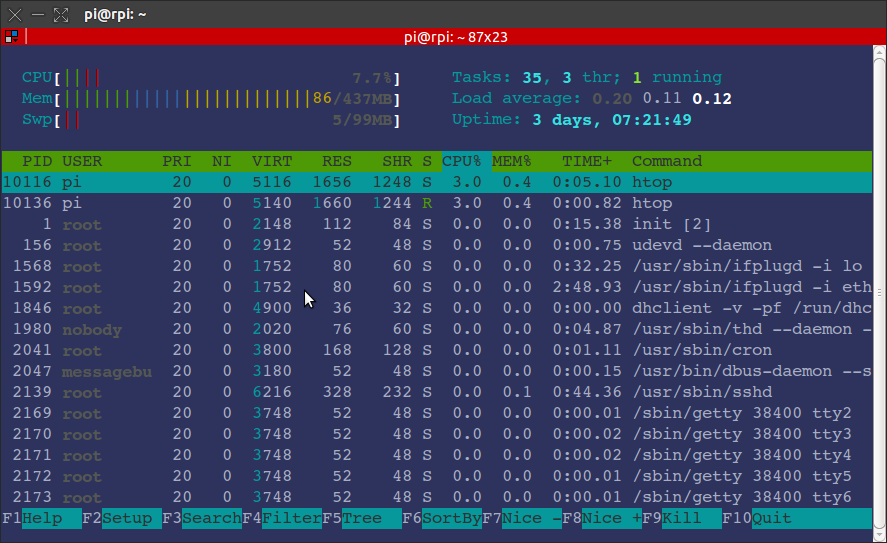
\includegraphics{htop.png}


\subsubsection{Enlarging the Swap Capacity}
\label{00_basic_config:enlarging-the-swap-capacity}
The typical RPi comes with 512 MB of memory only. This might not be enough in certain scenarios. One way to increase the memory (if only virtually) is to work with a larger than normal \textbf{swap partition}. The following steps generate a \textbf{1 GB} swap partition for the RPi.

First, make a \textbf{swap directory and swap file}:

\begin{Verbatim}[commandchars=\\\{\}]
sudo mkdir /media/swap
sudo dd if=/dev/zero of=/media/swap/swapfile.img bs=1024 count=1M
\end{Verbatim}

Second, generate the \textbf{swap filesystem}:
\begin{quote}

sudo mkswap /media/swap/swapfile.img
\end{quote}

Third, \textbf{edit} the following file:

\begin{Verbatim}[commandchars=\\\{\}]
sudo nano /etc/fstab
\end{Verbatim}

\textbf{Add} this line to that file:

\begin{Verbatim}[commandchars=\\\{\}]
/media/swap/swapfile.img swap swap sw 0 0
\end{Verbatim}

Fourth, \textbf{activate} the swap file:

\begin{Verbatim}[commandchars=\\\{\}]
sudo swapon /media/swap/swapfile.img
\end{Verbatim}

Finally, you can \textbf{check} whether the new swap configuration is indeed active---either via htop or as follws:

\begin{Verbatim}[commandchars=\\\{\}]
pi@rpi \PYGZti{} \PYGZdl{} cat /proc/swaps
Filename                                Type            Size    Used    Priority
/var/swap                               file            102396  6064    \PYGZhy{}1
/media/swap/swapfile.img                file            1048572 0       \PYGZhy{}2
pi@rpi \PYGZti{} \PYGZdl{}
\end{Verbatim}


\section{Raspberry Pi as FTP Server}
\label{01_ftp_server:raspberry-pi-as-ftp-server}\label{01_ftp_server::doc}
Setting up the RPi as an FTP server---over which you and you alone have full control---is quite a simple task. First, install the \code{ProFTP} software through:

\begin{Verbatim}[commandchars=\\\{\}]
sudo apt\PYGZhy{}get install proftpd
\end{Verbatim}

Configure it to be ``standalone''. Second, \textbf{edit the config file} of the program as follows:

\begin{Verbatim}[commandchars=\\\{\}]
sudo nano /etc/proftpd/proftpd.conf
\end{Verbatim}

Add the following \textbf{parameters}:

\begin{Verbatim}[commandchars=\\\{\}]
DefaultRoot         \PYGZti{}
AuthOrder           mod\PYGZus{}auth\PYGZus{}file.c  mod\PYGZus{}auth\PYGZus{}unix.c
AuthUserFile        /etc/proftpd/ftpd.passwd
AuthPAM             off
RequireValidShell   off
\end{Verbatim}

\textbf{Restart} the service by:

\begin{Verbatim}[commandchars=\\\{\}]
sudo /etc/init.d/proftpd restart
\end{Verbatim}

Third, \textbf{generate a new user} as follows:

\begin{Verbatim}[commandchars=\\\{\}]
sudo adduser ftp \PYGZhy{}\PYGZhy{}home /home/ftp \PYGZhy{}\PYGZhy{}shell /bin/bash
\end{Verbatim}

Change \code{ftp} and \code{/home/ftp} to a user name and directory of your liking. Choose a password for the new user.

Using a \textbf{FTP client}, you can now connect to your RPi and, for example, store files on it. You can also \code{ssh} connect to the RPi using the new user credentials.

Generally SD cards hosting the OS of the RPi and serving as file/data storage are of course not that large. But investing e.g. \textbf{50 EUR for a 500 GB external USB drive} and connecting such a drive to the RPi is a simple way of using the RPi as a serious \code{ftp} server.


\section{Raspberry Pi for Data Analytics}
\label{02_data_analytics:raspberry-pi-for-data-analytics}\label{02_data_analytics::doc}
This example is about data analytics with Python (cf. \href{http://python.org}{http://python.org}) and IPython (cf. \href{http://ipython.org}{http://ipython.org}) on the RPi. Before we install it, first install the Python PIP installer by:

\begin{Verbatim}[commandchars=\\\{\}]
sudo apt\PYGZhy{}get install python\PYGZhy{}pip python\PYGZhy{}dev build\PYGZhy{}essential
\end{Verbatim}


\subsection{Installing Data Analytics Libraries}
\label{02_data_analytics:installing-data-analytics-libraries}
Any serious data analytics effort with Python generally includes to some extent the \textbf{pandas} library (cf. \href{http://pandas.pydata.org}{http://pandas.pydata.org}). To install it, \textbf{upgrade the NumPy} library first (cf. \href{http://scipy.org}{http://scipy.org}):

\begin{Verbatim}[commandchars=\\\{\}]
sudo pip install numpy \PYGZhy{}\PYGZhy{}upgrade
\end{Verbatim}

This might take quite a while (1h+) due to the library being pretty large and the RPi not being that quick in compiling it. Then \textbf{install pandas}:

\begin{Verbatim}[commandchars=\\\{\}]
sudo pip install pandas
\end{Verbatim}

This also takes some time (again 1h+). Also install the \textbf{matplotlib} plotting library (with some updates/dependencies) as follows:

\begin{Verbatim}[commandchars=\\\{\}]
sudo easy\PYGZus{}install \PYGZhy{}U distribute
sudo apt\PYGZhy{}get install libpng\PYGZhy{}dev libjpeg8\PYGZhy{}dev libfreetype6\PYGZhy{}dev
sudo pip install matplotlib
\end{Verbatim}

And, oh wonder, this also takes quite a while to install and compile. We might want to install another useful library, namely \textbf{PyTables} (cf. \href{http://pytables.org}{http://pytables.org}) for efficient I/O with Python:

\begin{Verbatim}[commandchars=\\\{\}]
sudo pip install numexpr
sudo pip install cython
sudo apt\PYGZhy{}get install libhdf5\PYGZhy{}serial\PYGZhy{}dev
sudo pip install tables
\end{Verbatim}

All this taken together takes a few hours in total. However, your patience will pay off: your RPi will be equipped with \textbf{state-of-the-art Python-based data analytics libraries} that can be used then for a wide range of data collection, crunching and storage tasks. Finally, install the IPython interactive analytics environment:

\begin{Verbatim}[commandchars=\\\{\}]
sudo pip install ipython
\end{Verbatim}


\subsection{Interactive Data Analytics}
\label{02_data_analytics:interactive-data-analytics}
Now \textbf{start IPython} on the shell via:

\begin{Verbatim}[commandchars=\\\{\}]
\PYG{n}{ipython}
\end{Verbatim}

You should then see something like:

\begin{Verbatim}[commandchars=\\\{\}]
pi@rpi /home/ftp \PYGZdl{} ipython
Python 2.7.3 (default, Mar 18 2014, 05:13:23)
Type \PYGZdq{}copyright\PYGZdq{}, \PYGZdq{}credits\PYGZdq{} or \PYGZdq{}license\PYGZdq{} for more information.

IPython 2.3.1 \PYGZhy{}\PYGZhy{} An enhanced Interactive Python.
?         \PYGZhy{}\PYGZgt{} Introduction and overview of IPython\PYGZsq{}s features.
\PYGZpc{}quickref \PYGZhy{}\PYGZgt{} Quick reference.
help      \PYGZhy{}\PYGZgt{} Python\PYGZsq{}s own help system.
object?   \PYGZhy{}\PYGZgt{} Details about \PYGZsq{}object\PYGZsq{}, use \PYGZsq{}object??\PYGZsq{} for extra details.

In [1]:
\end{Verbatim}

Now let's retrieve some \textbf{stock quotes for the Apple stock}:

\begin{Verbatim}[commandchars=\\\{\}]
\PYG{g+gp}{In [1]: }\PYG{k+kn}{import} \PYG{n+nn}{pandas.io.data} \PYG{k+kn}{as} \PYG{n+nn}{web}

\PYG{g+gp}{In [2]: }\PYG{n}{aapl} \PYG{o}{=} \PYG{n}{web}\PYG{o}{.}\PYG{n}{DataReader}\PYG{p}{(}\PYG{l+s}{\PYGZsq{}}\PYG{l+s}{AAPL}\PYG{l+s}{\PYGZsq{}}\PYG{p}{,} \PYG{n}{data\PYGZus{}source}\PYG{o}{=}\PYG{l+s}{\PYGZsq{}}\PYG{l+s}{yahoo}\PYG{l+s}{\PYGZsq{}}\PYG{p}{)}

\PYG{g+gp}{In [3]: }\PYG{n}{aapl}\PYG{o}{.}\PYG{n}{tail}\PYG{p}{(}\PYG{p}{)}
\PYG{g+gh}{Out[3]: }
\PYG{g+go}{              Open    High     Low   Close    Volume  Adj Close}
\PYG{g+go}{Date                                                           }
\PYG{g+go}{2014\PYGZhy{}12\PYGZhy{}18  111.87  112.65  110.66  112.65  59006200     112.65}
\PYG{g+go}{2014\PYGZhy{}12\PYGZhy{}19  112.26  113.24  111.66  111.78  88429800     111.78}
\PYG{g+go}{2014\PYGZhy{}12\PYGZhy{}22  112.16  113.49  111.97  112.94  45167500     112.94}
\PYG{g+go}{2014\PYGZhy{}12\PYGZhy{}23  113.23  113.33  112.46  112.54  26028400     112.54}
\PYG{g+go}{2014\PYGZhy{}12\PYGZhy{}24  112.58  112.71  112.01  112.01  14460200     112.01}
\end{Verbatim}

Next, let us caculate two different \textbf{moving averages} (42 days \& 252 days):

\begin{Verbatim}[commandchars=\\\{\}]
\PYG{g+gp}{In [4]: }\PYG{k+kn}{import} \PYG{n+nn}{pandas} \PYG{k+kn}{as} \PYG{n+nn}{pd}

\PYG{g+gp}{In [5]: }\PYG{n}{aapl}\PYG{p}{[}\PYG{l+s}{\PYGZsq{}}\PYG{l+s}{42d}\PYG{l+s}{\PYGZsq{}}\PYG{p}{]} \PYG{o}{=} \PYG{n}{pd}\PYG{o}{.}\PYG{n}{rolling\PYGZus{}mean}\PYG{p}{(}\PYG{n}{aapl}\PYG{p}{[}\PYG{l+s}{\PYGZsq{}}\PYG{l+s}{Adj Close}\PYG{l+s}{\PYGZsq{}}\PYG{p}{]}\PYG{p}{,} \PYG{n}{window}\PYG{o}{=}\PYG{l+m+mi}{42}\PYG{p}{)}

\PYG{g+gp}{In [6]: }\PYG{n}{aapl}\PYG{p}{[}\PYG{l+s}{\PYGZsq{}}\PYG{l+s}{252d}\PYG{l+s}{\PYGZsq{}}\PYG{p}{]} \PYG{o}{=} \PYG{n}{pd}\PYG{o}{.}\PYG{n}{rolling\PYGZus{}mean}\PYG{p}{(}\PYG{n}{aapl}\PYG{p}{[}\PYG{l+s}{\PYGZsq{}}\PYG{l+s}{Adj Close}\PYG{l+s}{\PYGZsq{}}\PYG{p}{]}\PYG{p}{,} \PYG{n}{window}\PYG{o}{=}\PYG{l+m+mi}{252}\PYG{p}{)}
\end{Verbatim}

Finally, a plot of the index closing values and the moving averages:

\begin{Verbatim}[commandchars=\\\{\}]
\PYG{g+gp}{In [7]: }\PYG{k+kn}{import} \PYG{n+nn}{matplotlib.pyplot} \PYG{k+kn}{as} \PYG{n+nn}{plt}

\PYG{g+gp}{In [8]: }\PYG{n}{aapl}\PYG{p}{[}\PYG{p}{[}\PYG{l+s}{\PYGZsq{}}\PYG{l+s}{Adj Close}\PYG{l+s}{\PYGZsq{}}\PYG{p}{,} \PYG{l+s}{\PYGZsq{}}\PYG{l+s}{42d}\PYG{l+s}{\PYGZsq{}}\PYG{p}{,} \PYG{l+s}{\PYGZsq{}}\PYG{l+s}{252d}\PYG{l+s}{\PYGZsq{}}\PYG{p}{]}\PYG{p}{]}\PYG{o}{.}\PYG{n}{plot}\PYG{p}{(}\PYG{n}{title}\PYG{o}{=}\PYG{l+s}{\PYGZsq{}}\PYG{l+s}{Apple Inc.}\PYG{l+s}{\PYGZsq{}}\PYG{p}{)}\PYG{p}{;} \PYG{n}{plt}\PYG{o}{.}\PYG{n}{savefig}\PYG{p}{(}\PYG{l+s}{\PYGZsq{}}\PYG{l+s}{source/aapl.png}\PYG{l+s}{\PYGZsq{}}\PYG{p}{)}
\end{Verbatim}

The \textbf{saved png plot} might then look like below.

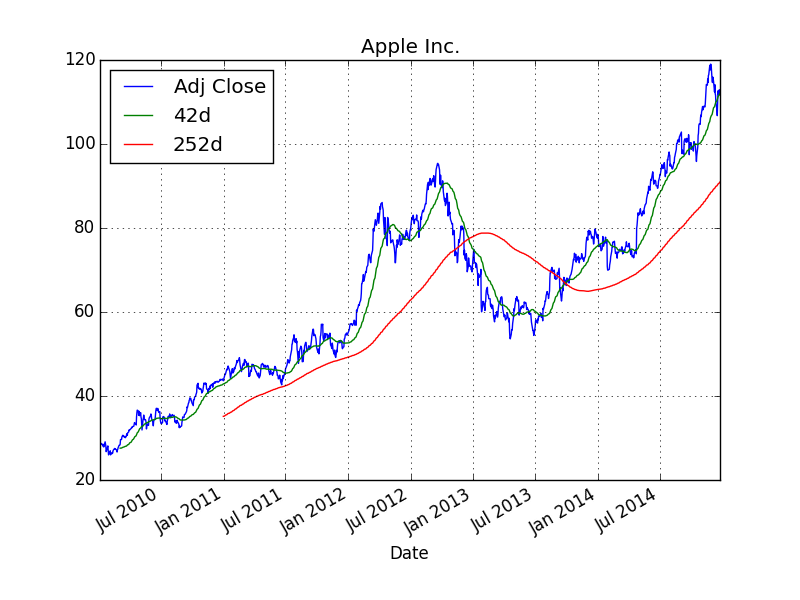
\includegraphics{aapl.png}

Via the shell (either directly or via \code{ssh} access) such figures cannot be displayed. However, you could imagine to run a Web site on the RPi where the figure is included and displayed via html (see {\hyperref[03_web_apps:web-apps]{\emph{Web Apps with Raspberry Pi}}}). You could also send such a graphical output/result to yourself or someone else e.g. by email or FTP transfer.


\subsection{Fast I/O Operations}
\label{02_data_analytics:fast-i-o-operations}
When using the RPi for data collection purposes, it might be beneficial to have efficient I/O capabilities available. This is where the PyTables library comes into play. The following is a Python script (\code{download link}) that collects stock data for a number of symbols and stores the data on disk in HDF5 format (cf. \href{http://hdfgroup.org}{http://hdfgroup.org}).

\begin{Verbatim}[commandchars=\\\{\}]
\PYG{c}{\PYGZsh{}}
\PYG{c}{\PYGZsh{} Collecting and Storing Stock Price Data}
\PYG{c}{\PYGZsh{} with Python/pandas/PyTables}
\PYG{c}{\PYGZsh{}}
\PYG{c}{\PYGZsh{} (c) Dr. Yves J. Hilpisch}
\PYG{c}{\PYGZsh{} The Python Quants GmbH}
\PYG{c}{\PYGZsh{} }
\PYG{k+kn}{import} \PYG{n+nn}{os}
\PYG{k+kn}{from} \PYG{n+nn}{time} \PYG{k+kn}{import} \PYG{n}{time}
\PYG{k+kn}{import} \PYG{n+nn}{pandas} \PYG{k+kn}{as} \PYG{n+nn}{pd}
\PYG{k+kn}{import} \PYG{n+nn}{pandas.io.data} \PYG{k+kn}{as} \PYG{n+nn}{web}

\PYG{n}{symbols} \PYG{o}{=} \PYG{p}{[}\PYG{l+s}{\PYGZsq{}}\PYG{l+s}{AAPL}\PYG{l+s}{\PYGZsq{}}\PYG{p}{,} \PYG{l+s}{\PYGZsq{}}\PYG{l+s}{YHOO}\PYG{l+s}{\PYGZsq{}}\PYG{p}{,} \PYG{l+s}{\PYGZsq{}}\PYG{l+s}{MSFT}\PYG{l+s}{\PYGZsq{}}\PYG{p}{]}

\PYG{n}{filename} \PYG{o}{=} \PYG{l+s}{\PYGZsq{}}\PYG{l+s}{data.h5}\PYG{l+s}{\PYGZsq{}}

\PYG{c}{\PYGZsh{}}
\PYG{c}{\PYGZsh{} Collecting the data}
\PYG{c}{\PYGZsh{}}
\PYG{n}{t0} \PYG{o}{=} \PYG{n}{time}\PYG{p}{(}\PYG{p}{)}
\PYG{n}{store} \PYG{o}{=} \PYG{p}{\PYGZob{}}\PYG{p}{\PYGZcb{}}  \PYG{c}{\PYGZsh{} dictionary to store DataFrame objects}

\PYG{k}{for} \PYG{n}{sym} \PYG{o+ow}{in} \PYG{n}{symbols}\PYG{p}{:}
    \PYG{n}{store}\PYG{p}{[}\PYG{n}{sym}\PYG{p}{]} \PYG{o}{=} \PYG{n}{web}\PYG{o}{.}\PYG{n}{DataReader}\PYG{p}{(}\PYG{n}{sym}\PYG{p}{,} \PYG{n}{data\PYGZus{}source}\PYG{o}{=}\PYG{l+s}{\PYGZsq{}}\PYG{l+s}{yahoo}\PYG{l+s}{\PYGZsq{}}\PYG{p}{,} \PYG{n}{start}\PYG{o}{=}\PYG{l+s}{\PYGZsq{}}\PYG{l+s}{2000/1/1}\PYG{l+s}{\PYGZsq{}}\PYG{p}{)}

\PYG{c}{\PYGZsh{}}
\PYG{c}{\PYGZsh{} Storing data in HDF5 database}
\PYG{c}{\PYGZsh{}}
\PYG{n}{t1} \PYG{o}{=} \PYG{n}{time}\PYG{p}{(}\PYG{p}{)}

\PYG{n}{h5} \PYG{o}{=} \PYG{n}{pd}\PYG{o}{.}\PYG{n}{HDFStore}\PYG{p}{(}\PYG{n}{filename}\PYG{p}{,} \PYG{l+s}{\PYGZsq{}}\PYG{l+s}{w}\PYG{l+s}{\PYGZsq{}}\PYG{p}{)}  \PYG{c}{\PYGZsh{} open database file}

\PYG{k}{for} \PYG{n}{sym} \PYG{o+ow}{in} \PYG{n}{symbols}\PYG{p}{:}
    \PYG{n}{h5}\PYG{p}{[}\PYG{n}{sym}\PYG{p}{]} \PYG{o}{=} \PYG{n}{store}\PYG{p}{[}\PYG{n}{sym}\PYG{p}{]}  \PYG{c}{\PYGZsh{} write DataFrame to disk}

\PYG{n}{h5}\PYG{o}{.}\PYG{n}{close}\PYG{p}{(}\PYG{p}{)}  \PYG{c}{\PYGZsh{} close database}

\PYG{n}{t2} \PYG{o}{=} \PYG{n}{time}\PYG{p}{(}\PYG{p}{)}
\PYG{n}{os}\PYG{o}{.}\PYG{n}{remove}\PYG{p}{(}\PYG{n}{filename}\PYG{p}{)}  \PYG{c}{\PYGZsh{} delete file on disk}
\PYG{c}{\PYGZsh{}}
\PYG{c}{\PYGZsh{} Output}
\PYG{c}{\PYGZsh{}}
\PYG{k}{print} \PYG{l+s}{\PYGZdq{}}\PYG{l+s}{Time needed to collect data in sec. }\PYG{l+s+si}{\PYGZpc{}5.2f}\PYG{l+s}{\PYGZdq{}} \PYG{o}{\PYGZpc{}} \PYG{p}{(}\PYG{n}{t1} \PYG{o}{\PYGZhy{}} \PYG{n}{t0}\PYG{p}{)}
\PYG{k}{print} \PYG{l+s}{\PYGZdq{}}\PYG{l+s}{Time needed to store data in sec.   }\PYG{l+s+si}{\PYGZpc{}5.2f}\PYG{l+s}{\PYGZdq{}} \PYG{o}{\PYGZpc{}} \PYG{p}{(}\PYG{n}{t2} \PYG{o}{\PYGZhy{}} \PYG{n}{t1}\PYG{p}{)}
\end{Verbatim}

Running the script from the shell yields an output like this:

\begin{Verbatim}[commandchars=\\\{\}]
pi@rpi \PYGZti{} \PYGZdl{} python data\PYGZus{}collection.py
Time needed to collect data in sec.  1.61
Time needed to store data in sec.    1.40
\end{Verbatim}

The data gathered and stored by this Python script is not that large. The following script (\code{download link}) generates a set with pseudo-random sample data which is \textbf{80 MB in size} and writes it to disk.

\begin{Verbatim}[commandchars=\\\{\}]
\PYG{c}{\PYGZsh{}}
\PYG{c}{\PYGZsh{} Storing a Larger Data Set on Disk}
\PYG{c}{\PYGZsh{} with Python/pandas/PyTables}
\PYG{c}{\PYGZsh{}}
\PYG{c}{\PYGZsh{} (c) Dr. Yves J. Hilpisch}
\PYG{c}{\PYGZsh{} The Python Quants GmbH}
\PYG{c}{\PYGZsh{} }
\PYG{k+kn}{import} \PYG{n+nn}{os}
\PYG{k+kn}{from} \PYG{n+nn}{time} \PYG{k+kn}{import} \PYG{n}{time}
\PYG{k+kn}{import} \PYG{n+nn}{numpy} \PYG{k+kn}{as} \PYG{n+nn}{np}
\PYG{k+kn}{import} \PYG{n+nn}{pandas} \PYG{k+kn}{as} \PYG{n+nn}{pd}

\PYG{n}{filename} \PYG{o}{=} \PYG{l+s}{\PYGZsq{}}\PYG{l+s}{data.h5}\PYG{l+s}{\PYGZsq{}}

\PYG{c}{\PYGZsh{}}
\PYG{c}{\PYGZsh{} Generating the sample data}
\PYG{c}{\PYGZsh{}}
\PYG{n}{t0} \PYG{o}{=} \PYG{n}{time}\PYG{p}{(}\PYG{p}{)}

\PYG{n}{data} \PYG{o}{=} \PYG{n}{np}\PYG{o}{.}\PYG{n}{random}\PYG{o}{.}\PYG{n}{standard\PYGZus{}normal}\PYG{p}{(}\PYG{l+m+mi}{10000000}\PYG{p}{)}  \PYG{c}{\PYGZsh{} random data}

\PYG{n}{df} \PYG{o}{=} \PYG{n}{pd}\PYG{o}{.}\PYG{n}{DataFrame}\PYG{p}{(}\PYG{n}{data}\PYG{p}{)}  \PYG{c}{\PYGZsh{} pandas DataFrame object}

\PYG{c}{\PYGZsh{}}
\PYG{c}{\PYGZsh{} Storing data in HDF5 database}
\PYG{c}{\PYGZsh{}}
\PYG{n}{t1} \PYG{o}{=} \PYG{n}{time}\PYG{p}{(}\PYG{p}{)}

\PYG{n}{h5} \PYG{o}{=} \PYG{n}{pd}\PYG{o}{.}\PYG{n}{HDFStore}\PYG{p}{(}\PYG{n}{filename}\PYG{p}{,} \PYG{l+s}{\PYGZsq{}}\PYG{l+s}{w}\PYG{l+s}{\PYGZsq{}}\PYG{p}{)}  \PYG{c}{\PYGZsh{} open database file}
\PYG{n}{h5}\PYG{p}{[}\PYG{l+s}{\PYGZsq{}}\PYG{l+s}{data}\PYG{l+s}{\PYGZsq{}}\PYG{p}{]} \PYG{o}{=} \PYG{n}{df}  \PYG{c}{\PYGZsh{} write DataFrame to disk}
\PYG{n}{h5}\PYG{o}{.}\PYG{n}{close}\PYG{p}{(}\PYG{p}{)}  \PYG{c}{\PYGZsh{} close database file}

\PYG{n}{t2} \PYG{o}{=} \PYG{n}{time}\PYG{p}{(}\PYG{p}{)}
\PYG{n}{os}\PYG{o}{.}\PYG{n}{remove}\PYG{p}{(}\PYG{n}{filename}\PYG{p}{)}  \PYG{c}{\PYGZsh{} delete file on disk}
\PYG{c}{\PYGZsh{}}
\PYG{c}{\PYGZsh{} Output}
\PYG{c}{\PYGZsh{}}
\PYG{k}{print} \PYG{l+s}{\PYGZdq{}}\PYG{l+s}{Size of data set in bytes }\PYG{l+s+si}{\PYGZpc{}d}\PYG{l+s}{\PYGZdq{}} \PYG{o}{\PYGZpc{}} \PYG{n}{data}\PYG{o}{.}\PYG{n}{nbytes}
\PYG{k}{print} \PYG{l+s}{\PYGZdq{}}\PYG{l+s}{Time needed to generate data in sec. }\PYG{l+s+si}{\PYGZpc{}5.2f}\PYG{l+s}{\PYGZdq{}} \PYG{o}{\PYGZpc{}} \PYG{p}{(}\PYG{n}{t1} \PYG{o}{\PYGZhy{}} \PYG{n}{t0}\PYG{p}{)}
\PYG{k}{print} \PYG{l+s}{\PYGZdq{}}\PYG{l+s}{Time needed to store data in sec.    }\PYG{l+s+si}{\PYGZpc{}5.2f}\PYG{l+s}{\PYGZdq{}} \PYG{o}{\PYGZpc{}} \PYG{p}{(}\PYG{n}{t2} \PYG{o}{\PYGZhy{}} \PYG{n}{t1}\PYG{p}{)}
\end{Verbatim}

Running this script yields an output like follows:

\begin{Verbatim}[commandchars=\\\{\}]
pi@rpi \PYGZti{} \PYGZdl{} python large\PYGZus{}data\PYGZus{}set.py
Size of data set in bytes 80000000
Time needed to generate data in sec. 10.24
Time needed to store data in sec.     9.39
\end{Verbatim}

It takes less than 10 seconds to write 80 MB of data to the SD card (times here might vary significantly depending on the card type used). You see that you can even process \textbf{larger data sets} (although not ``big data'') with the  RPi.


\section{Web Apps with Raspberry Pi}
\label{03_web_apps:web-apps-with-raspberry-pi}\label{03_web_apps:web-apps}\label{03_web_apps::doc}
Having implemented the small project about data analytics with Python, we are now well equipped to do something useful with the data analytics capabilities. In particular, we want to build a small \textbf{Web app} that serves a page where you can decide on a ticker symbol and you get back historical stock price data for that symbol.

The framework we are going to use is called \textbf{Flask} (cf. \href{http://flask.pocoo.org/}{http://flask.pocoo.org/}) and has become quite popular recently in the Python world. Installation in this case is straightforward:

\begin{Verbatim}[commandchars=\\\{\}]
sudo pip install Flask
sudo pip install flask\PYGZhy{}wtf
\end{Verbatim}

To get our Web app to be build served, we need a \textbf{Web server}. A popular choice in the Python world is \textbf{Tornado} (cf. \href{http://www.tornadoweb.org/en/stable/}{http://www.tornadoweb.org/en/stable/}). Install it via:

\begin{Verbatim}[commandchars=\\\{\}]
sudo pip install tornado
\end{Verbatim}

This should also be quick and straightforward. This is almost all we need to use the RPi as a Web server for Web sites or applications.


\subsection{A First Example}
\label{03_web_apps:a-first-example}
Let us see if we can implement the \textbf{``Hello World!'' example} of Flask and get it served with Tornado. First the Web app itself:

\begin{Verbatim}[commandchars=\\\{\}]
\PYG{c}{\PYGZsh{}}
\PYG{c}{\PYGZsh{} From http://flask.pocoo.org}
\PYG{c}{\PYGZsh{}}
\PYG{k+kn}{from} \PYG{n+nn}{flask} \PYG{k+kn}{import} \PYG{n}{Flask} 
\PYG{n}{app} \PYG{o}{=} \PYG{n}{Flask}\PYG{p}{(}\PYG{n}{\PYGZus{}\PYGZus{}name\PYGZus{}\PYGZus{}}\PYG{p}{)}

\PYG{n+nd}{@app.route}\PYG{p}{(}\PYG{l+s}{\PYGZdq{}}\PYG{l+s}{/}\PYG{l+s}{\PYGZdq{}}\PYG{p}{)}
\PYG{k}{def} \PYG{n+nf}{hello}\PYG{p}{(}\PYG{p}{)}\PYG{p}{:}
    \PYG{k}{return} \PYG{l+s}{\PYGZdq{}}\PYG{l+s}{Hello World!}\PYG{l+s}{\PYGZdq{}}
\end{Verbatim}

As you see, a few lines of code suffice for a propor Web application---even if it is only a very small one. The \code{download link} for this Python module.

Next, we need to wrap the app into a \textbf{WSGI container} (cf. \href{http://en.wikipedia.org/wiki/Web\_Server\_Gateway\_Interface}{http://en.wikipedia.org/wiki/Web\_Server\_Gateway\_Interface}) to be served by Tornado:

\begin{Verbatim}[commandchars=\\\{\}]
\PYG{c}{\PYGZsh{}}
\PYG{c}{\PYGZsh{} From http://flask.pocoo.org}
\PYG{c}{\PYGZsh{}}
\PYG{k+kn}{from} \PYG{n+nn}{tornado.wsgi} \PYG{k+kn}{import} \PYG{n}{WSGIContainer}
\PYG{k+kn}{from} \PYG{n+nn}{tornado.httpserver} \PYG{k+kn}{import} \PYG{n}{HTTPServer}
\PYG{k+kn}{from} \PYG{n+nn}{tornado.ioloop} \PYG{k+kn}{import} \PYG{n}{IOLoop}
\PYG{k+kn}{from} \PYG{n+nn}{flask\PYGZus{}test} \PYG{k+kn}{import} \PYG{n}{app}

\PYG{n}{http\PYGZus{}server} \PYG{o}{=} \PYG{n}{HTTPServer}\PYG{p}{(}\PYG{n}{WSGIContainer}\PYG{p}{(}\PYG{n}{app}\PYG{p}{)}\PYG{p}{)}
\PYG{n}{http\PYGZus{}server}\PYG{o}{.}\PYG{n}{listen}\PYG{p}{(}\PYG{l+m+mi}{5000}\PYG{p}{)}  \PYG{c}{\PYGZsh{} serving on port 5000}
\PYG{n}{IOLoop}\PYG{o}{.}\PYG{n}{instance}\PYG{p}{(}\PYG{p}{)}\PYG{o}{.}\PYG{n}{start}\PYG{p}{(}\PYG{p}{)}
\end{Verbatim}

Again only a few lines of code. The \code{download link} for this script. If you execute this last script via:

\begin{Verbatim}[commandchars=\\\{\}]
python web\PYGZus{}serve.py
\end{Verbatim}

you should be able to see the result when going to the \textbf{fixed IP or domain of your RPi} in combination with port 5000 (cf. {\hyperref[00_basic_config:fixip]{\emph{Fixed IP Address}}}):

\begin{Verbatim}[commandchars=\\\{\}]
http://xx.yy.zz.100:5000
\end{Verbatim}

or:

\begin{Verbatim}[commandchars=\\\{\}]
http://rpi.mydomain.net:5000
\end{Verbatim}


\subsection{Historical Stock Price Data}
\label{03_web_apps:historical-stock-price-data}
This Web application retrieves historical stock price data for a user given \textbf{ticker symbol} and calculates \textbf{two different trends (moving averages)}. It then outputs a figure with the data and results as well as a HTML table with the raw data.

Let us start with the \textbf{Web app code} itself:

\begin{Verbatim}[commandchars=\\\{\}]
\PYG{c}{\PYGZsh{}}
\PYG{c}{\PYGZsh{} Historical Stock Prices}
\PYG{c}{\PYGZsh{} with the RPi using Python \PYGZam{} Flask}
\PYG{c}{\PYGZsh{}}
\PYG{c}{\PYGZsh{} stock\PYGZus{}data.py}
\PYG{c}{\PYGZsh{}}
\PYG{c}{\PYGZsh{} (c) Dr. Yves J. Hilpisch}
\PYG{c}{\PYGZsh{} The Python Quants}
\PYG{c}{\PYGZsh{}}

\PYG{k+kn}{import} \PYG{n+nn}{pandas} \PYG{k+kn}{as} \PYG{n+nn}{pd}
\PYG{k+kn}{import} \PYG{n+nn}{pandas.io.data} \PYG{k+kn}{as} \PYG{n+nn}{web}
\PYG{k+kn}{import} \PYG{n+nn}{matplotlib.pyplot} \PYG{k+kn}{as} \PYG{n+nn}{plt}
\PYG{k+kn}{from} \PYG{n+nn}{flask} \PYG{k+kn}{import} \PYG{n}{Flask}\PYG{p}{,} \PYG{n}{request}\PYG{p}{,} \PYG{n}{render\PYGZus{}template}\PYG{p}{,} \PYG{n}{redirect}\PYG{p}{,} \PYG{n}{url\PYGZus{}for}
\PYG{k+kn}{from} \PYG{n+nn}{forms} \PYG{k+kn}{import} \PYG{n}{SymbolSearch}


\PYG{n}{app} \PYG{o}{=} \PYG{n}{Flask}\PYG{p}{(}\PYG{n}{\PYGZus{}\PYGZus{}name\PYGZus{}\PYGZus{}}\PYG{p}{)}

\PYG{n+nd}{@app.route}\PYG{p}{(}\PYG{l+s}{\PYGZdq{}}\PYG{l+s}{/}\PYG{l+s}{\PYGZdq{}}\PYG{p}{,} \PYG{n}{methods}\PYG{o}{=}\PYG{p}{[}\PYG{l+s}{\PYGZsq{}}\PYG{l+s}{GET}\PYG{l+s}{\PYGZsq{}}\PYG{p}{,} \PYG{l+s}{\PYGZsq{}}\PYG{l+s}{POST}\PYG{l+s}{\PYGZsq{}}\PYG{p}{]}\PYG{p}{)}
\PYG{k}{def} \PYG{n+nf}{main}\PYG{p}{(}\PYG{p}{)}\PYG{p}{:}
    \PYG{n}{form} \PYG{o}{=} \PYG{n}{SymbolSearch}\PYG{p}{(}\PYG{n}{csrf\PYGZus{}enabled}\PYG{o}{=}\PYG{n+nb+bp}{False}\PYG{p}{)}
    \PYG{k}{if} \PYG{n}{request}\PYG{o}{.}\PYG{n}{method} \PYG{o}{==} \PYG{l+s}{\PYGZsq{}}\PYG{l+s}{POST}\PYG{l+s}{\PYGZsq{}}\PYG{p}{:}
        \PYG{k}{return} \PYG{n}{redirect}\PYG{p}{(}\PYG{n}{url\PYGZus{}for}\PYG{p}{(}\PYG{l+s}{\PYGZsq{}}\PYG{l+s}{results}\PYG{l+s}{\PYGZsq{}}\PYG{p}{,} \PYG{n}{symbol}\PYG{o}{=}\PYG{n}{request}\PYG{o}{.}\PYG{n}{form}\PYG{p}{[}\PYG{l+s}{\PYGZsq{}}\PYG{l+s}{symbol}\PYG{l+s}{\PYGZsq{}}\PYG{p}{]}\PYG{p}{,}
                            \PYG{n}{trend1}\PYG{o}{=}\PYG{n}{request}\PYG{o}{.}\PYG{n}{form}\PYG{p}{[}\PYG{l+s}{\PYGZsq{}}\PYG{l+s}{trend1}\PYG{l+s}{\PYGZsq{}}\PYG{p}{]}\PYG{p}{,}
                            \PYG{n}{trend2}\PYG{o}{=}\PYG{n}{request}\PYG{o}{.}\PYG{n}{form}\PYG{p}{[}\PYG{l+s}{\PYGZsq{}}\PYG{l+s}{trend2}\PYG{l+s}{\PYGZsq{}}\PYG{p}{]}\PYG{p}{)}\PYG{p}{)}
    \PYG{k}{return} \PYG{n}{render\PYGZus{}template}\PYG{p}{(}\PYG{l+s}{\PYGZsq{}}\PYG{l+s}{selection.html}\PYG{l+s}{\PYGZsq{}}\PYG{p}{,} \PYG{n}{form}\PYG{o}{=}\PYG{n}{form}\PYG{p}{)}

\PYG{n+nd}{@app.route}\PYG{p}{(}\PYG{l+s}{\PYGZdq{}}\PYG{l+s}{/symbol/\PYGZlt{}symbol\PYGZgt{}+\PYGZlt{}trend1\PYGZgt{}+\PYGZlt{}trend2\PYGZgt{}}\PYG{l+s}{\PYGZdq{}}\PYG{p}{)}
\PYG{k}{def} \PYG{n+nf}{results}\PYG{p}{(}\PYG{n}{symbol}\PYG{p}{,} \PYG{n}{trend1}\PYG{p}{,} \PYG{n}{trend2}\PYG{p}{)}\PYG{p}{:}
    \PYG{n}{data} \PYG{o}{=} \PYG{n}{web}\PYG{o}{.}\PYG{n}{DataReader}\PYG{p}{(}\PYG{n}{symbol}\PYG{p}{,} \PYG{n}{data\PYGZus{}source}\PYG{o}{=}\PYG{l+s}{\PYGZsq{}}\PYG{l+s}{yahoo}\PYG{l+s}{\PYGZsq{}}\PYG{p}{)}
    \PYG{n}{data}\PYG{p}{[}\PYG{l+s}{\PYGZsq{}}\PYG{l+s}{Trend 1}\PYG{l+s}{\PYGZsq{}}\PYG{p}{]} \PYG{o}{=} \PYG{n}{pd}\PYG{o}{.}\PYG{n}{rolling\PYGZus{}mean}\PYG{p}{(}\PYG{n}{data}\PYG{p}{[}\PYG{l+s}{\PYGZsq{}}\PYG{l+s}{Adj Close}\PYG{l+s}{\PYGZsq{}}\PYG{p}{]}\PYG{p}{,} \PYG{n}{window}\PYG{o}{=}\PYG{n+nb}{int}\PYG{p}{(}\PYG{n}{trend1}\PYG{p}{)}\PYG{p}{)}
    \PYG{n}{data}\PYG{p}{[}\PYG{l+s}{\PYGZsq{}}\PYG{l+s}{Trend 2}\PYG{l+s}{\PYGZsq{}}\PYG{p}{]} \PYG{o}{=} \PYG{n}{pd}\PYG{o}{.}\PYG{n}{rolling\PYGZus{}mean}\PYG{p}{(}\PYG{n}{data}\PYG{p}{[}\PYG{l+s}{\PYGZsq{}}\PYG{l+s}{Adj Close}\PYG{l+s}{\PYGZsq{}}\PYG{p}{]}\PYG{p}{,} \PYG{n}{window}\PYG{o}{=}\PYG{n+nb}{int}\PYG{p}{(}\PYG{n}{trend2}\PYG{p}{)}\PYG{p}{)}
    \PYG{n}{data}\PYG{p}{[}\PYG{p}{[}\PYG{l+s}{\PYGZsq{}}\PYG{l+s}{Adj Close}\PYG{l+s}{\PYGZsq{}}\PYG{p}{,} \PYG{l+s}{\PYGZsq{}}\PYG{l+s}{Trend 1}\PYG{l+s}{\PYGZsq{}}\PYG{p}{,} \PYG{l+s}{\PYGZsq{}}\PYG{l+s}{Trend 2}\PYG{l+s}{\PYGZsq{}}\PYG{p}{]}\PYG{p}{]}\PYG{o}{.}\PYG{n}{plot}\PYG{p}{(}\PYG{p}{)}
    \PYG{n}{output} \PYG{o}{=} \PYG{l+s}{\PYGZsq{}}\PYG{l+s}{results.png}\PYG{l+s}{\PYGZsq{}}
    \PYG{n}{plt}\PYG{o}{.}\PYG{n}{savefig}\PYG{p}{(}\PYG{l+s}{\PYGZsq{}}\PYG{l+s}{static/}\PYG{l+s}{\PYGZsq{}} \PYG{o}{+} \PYG{n}{output}\PYG{p}{)}
    \PYG{n}{table} \PYG{o}{=} \PYG{n}{data}\PYG{o}{.}\PYG{n}{to\PYGZus{}html}\PYG{p}{(}\PYG{p}{)}
    \PYG{k}{return} \PYG{n}{render\PYGZus{}template}\PYG{p}{(}\PYG{l+s}{\PYGZsq{}}\PYG{l+s}{results.html}\PYG{l+s}{\PYGZsq{}}\PYG{p}{,} \PYG{n}{symbol}\PYG{o}{=}\PYG{n}{symbol}\PYG{p}{,}
                            \PYG{n}{output}\PYG{o}{=}\PYG{n}{output}\PYG{p}{,} \PYG{n}{table}\PYG{o}{=}\PYG{n}{table}\PYG{p}{)}


\PYG{k}{if} \PYG{n}{\PYGZus{}\PYGZus{}name\PYGZus{}\PYGZus{}} \PYG{o}{==} \PYG{l+s}{\PYGZsq{}}\PYG{l+s}{\PYGZus{}\PYGZus{}main\PYGZus{}\PYGZus{}}\PYG{l+s}{\PYGZsq{}}\PYG{p}{:}
    \PYG{n}{app}\PYG{o}{.}\PYG{n}{run}\PYG{p}{(}\PYG{n}{debug}\PYG{o}{=}\PYG{n+nb+bp}{True}\PYG{p}{)}
\end{Verbatim}

The \code{download link} for this Python script.

We need a simple \textbf{WTF form} for data input (\code{download link})

\begin{Verbatim}[commandchars=\\\{\}]
\PYG{c}{\PYGZsh{}}
\PYG{c}{\PYGZsh{} Data input form}
\PYG{c}{\PYGZsh{} forms.py}
\PYG{c}{\PYGZsh{}}

\PYG{k+kn}{from} \PYG{n+nn}{wtforms} \PYG{k+kn}{import} \PYG{n}{TextField}
\PYG{k+kn}{from} \PYG{n+nn}{wtforms.fields} \PYG{k+kn}{import} \PYG{n}{SubmitField}
\PYG{k+kn}{from} \PYG{n+nn}{wtforms.validators} \PYG{k+kn}{import} \PYG{n}{DataRequired}
\PYG{k+kn}{from} \PYG{n+nn}{flask.ext.wtf} \PYG{k+kn}{import} \PYG{n}{Form}

\PYG{k}{class} \PYG{n+nc}{SymbolSearch}\PYG{p}{(}\PYG{n}{Form}\PYG{p}{)}\PYG{p}{:}
    \PYG{n}{symbol} \PYG{o}{=} \PYG{n}{TextField}\PYG{p}{(}\PYG{l+s}{\PYGZsq{}}\PYG{l+s}{Symbol}\PYG{l+s}{\PYGZsq{}}\PYG{p}{,} \PYG{n}{validators}\PYG{o}{=}\PYG{p}{[}\PYG{n}{DataRequired}\PYG{p}{,}\PYG{p}{]}\PYG{p}{)}
    \PYG{n}{trend1} \PYG{o}{=} \PYG{n}{TextField}\PYG{p}{(}\PYG{l+s}{\PYGZsq{}}\PYG{l+s}{Trend 1}\PYG{l+s}{\PYGZsq{}}\PYG{p}{,} \PYG{n}{validators}\PYG{o}{=}\PYG{p}{[}\PYG{n}{DataRequired}\PYG{p}{,}\PYG{p}{]}\PYG{p}{)}
    \PYG{n}{trend2} \PYG{o}{=} \PYG{n}{TextField}\PYG{p}{(}\PYG{l+s}{\PYGZsq{}}\PYG{l+s}{Trend 2}\PYG{l+s}{\PYGZsq{}}\PYG{p}{,} \PYG{n}{validators}\PYG{o}{=}\PYG{p}{[}\PYG{n}{DataRequired}\PYG{p}{,}\PYG{p}{]}\PYG{p}{)}
    \PYG{n}{submit} \PYG{o}{=} \PYG{n}{SubmitField}\PYG{p}{(}\PYG{l+s}{\PYGZsq{}}\PYG{l+s}{Search}\PYG{l+s}{\PYGZsq{}}\PYG{p}{)}
\end{Verbatim}

The major \textbf{layout template} (\code{download link}:

\begin{Verbatim}[commandchars=\\\{\}]
\PYG{c}{\PYGZlt{}!\PYGZhy{}\PYGZhy{}}\PYG{c}{ layout.html }\PYG{c}{\PYGZhy{}\PYGZhy{}\PYGZgt{}}
\PYG{c+cp}{\PYGZlt{}!doctype html\PYGZgt{}}
\PYG{n+nt}{\PYGZlt{}title}\PYG{n+nt}{\PYGZgt{}}Historical Stock Prices\PYG{n+nt}{\PYGZlt{}/title\PYGZgt{}}

\PYG{n+nt}{\PYGZlt{}head}\PYG{n+nt}{\PYGZgt{}}

\PYG{n+nt}{\PYGZlt{}/head\PYGZgt{}}

\PYG{n+nt}{\PYGZlt{}link} \PYG{n+na}{rel=}\PYG{l+s}{stylesheet} \PYG{n+na}{type=}\PYG{l+s}{text/css}
      \PYG{n+na}{href=}\PYG{l+s}{\PYGZdq{}\PYGZob{}\PYGZob{} url\PYGZus{}for(\PYGZsq{}static\PYGZsq{}, filename=\PYGZsq{}style.css\PYGZsq{}) \PYGZcb{}\PYGZcb{}\PYGZdq{}}\PYG{n+nt}{\PYGZgt{}}

\PYG{n+nt}{\PYGZlt{}link} \PYG{n+na}{href=}\PYG{l+s}{\PYGZsq{}http://fonts.googleapis.com/css?family=PT+Sans\PYGZsq{}}
      \PYG{n+na}{rel=}\PYG{l+s}{\PYGZsq{}stylesheet\PYGZsq{}} \PYG{n+na}{type=}\PYG{l+s}{\PYGZsq{}text/css\PYGZsq{}}\PYG{n+nt}{\PYGZgt{}}

\PYG{n+nt}{\PYGZlt{}link} \PYG{n+na}{rel=}\PYG{l+s}{\PYGZdq{}shortcut icon\PYGZdq{}}
      \PYG{n+na}{href=}\PYG{l+s}{\PYGZdq{}http://hilpisch.com/favicon.ico\PYGZdq{}}\PYG{n+nt}{\PYGZgt{}}

\PYG{n+nt}{\PYGZlt{}div} \PYG{n+na}{class=}\PYG{l+s}{page}\PYG{n+nt}{\PYGZgt{}}
  
  \PYG{n+nt}{\PYGZlt{}div} \PYG{n+na}{class=}\PYG{l+s}{logo}\PYG{n+nt}{\PYGZgt{}}
    \PYG{n+nt}{\PYGZlt{}img} \PYG{n+na}{src=}\PYG{l+s}{\PYGZsq{}http://hilpisch.com/tpq\PYGZus{}logo.png\PYGZsq{}} \PYG{n+na}{alt=}\PYG{l+s}{\PYGZdq{}TPQ Logo\PYGZdq{}}\PYG{n+nt}{\PYGZgt{}}
  \PYG{n+nt}{\PYGZlt{}/div\PYGZgt{}}
  
  \PYG{n+nt}{\PYGZlt{}div} \PYG{n+na}{class=}\PYG{l+s}{metanav}\PYG{n+nt}{\PYGZgt{}}
    \PYG{n+nt}{\PYGZlt{}a} \PYG{n+na}{href=}\PYG{l+s}{\PYGZdq{}\PYGZob{}\PYGZob{} url\PYGZus{}for(\PYGZsq{}main\PYGZsq{})\PYGZcb{}\PYGZcb{}\PYGZdq{}}\PYG{n+nt}{\PYGZgt{}}main\PYG{n+nt}{\PYGZlt{}/a\PYGZgt{}}
  \PYG{n+nt}{\PYGZlt{}/div\PYGZgt{}}
  \PYGZob{}\PYGZpc{} block body \PYGZpc{}\PYGZcb{}

  \PYGZob{}\PYGZpc{} endblock \PYGZpc{}\PYGZcb{}
\PYG{n+nt}{\PYGZlt{}/div\PYGZgt{}}
\end{Verbatim}

The sub-template for the \textbf{data input} (\code{download link}):

\begin{Verbatim}[commandchars=\\\{\}]
\PYG{c}{\PYGZlt{}!\PYGZhy{}\PYGZhy{}}\PYG{c}{ selection.html }\PYG{c}{\PYGZhy{}\PYGZhy{}\PYGZgt{}}
\PYGZob{}\PYGZpc{} extends \PYGZdq{}layout.html\PYGZdq{} \PYGZpc{}\PYGZcb{}

\PYGZob{}\PYGZpc{} macro render\PYGZus{}field(field) \PYGZpc{}\PYGZcb{}
  \PYG{n+nt}{\PYGZlt{}dd}\PYG{n+nt}{\PYGZgt{}}\PYGZob{}\PYGZob{} field.label \PYGZcb{}\PYGZcb{}
  \PYG{n+nt}{\PYGZlt{}dd}\PYG{n+nt}{\PYGZgt{}}\PYGZob{}\PYGZob{} field(**kwargs)\textbar{}safe \PYGZcb{}\PYGZcb{}
  \PYGZob{}\PYGZpc{} if field.errors \PYGZpc{}\PYGZcb{}
    \PYG{n+nt}{\PYGZlt{}ul} \PYG{n+na}{class=}\PYG{l+s}{errors}\PYG{n+nt}{\PYGZgt{}}
    \PYGZob{}\PYGZpc{} for error in field.errors \PYGZpc{}\PYGZcb{}
      \PYG{n+nt}{\PYGZlt{}dd}\PYG{n+nt}{\PYGZgt{}}\PYGZob{}\PYGZob{} error \PYGZcb{}\PYGZcb{}\PYG{n+nt}{\PYGZlt{}/dd\PYGZgt{}}
    \PYGZob{}\PYGZpc{} endfor \PYGZpc{}\PYGZcb{}
    \PYG{n+nt}{\PYGZlt{}/ul\PYGZgt{}}
  \PYGZob{}\PYGZpc{} endif \PYGZpc{}\PYGZcb{}
  \PYG{n+nt}{\PYGZlt{}/dd\PYGZgt{}}
\PYGZob{}\PYGZpc{} endmacro \PYGZpc{}\PYGZcb{}

\PYGZob{}\PYGZpc{} block body \PYGZpc{}\PYGZcb{}

  \PYG{n+nt}{\PYGZlt{}form} \PYG{n+na}{action=}\PYG{l+s}{\PYGZdq{}\PYGZob{}\PYGZob{} url\PYGZus{}for(\PYGZsq{}main\PYGZsq{}) \PYGZcb{}\PYGZcb{}\PYGZdq{}} \PYG{n+na}{method=}\PYG{l+s}{post}
   \PYG{n+na}{enctype=}\PYG{l+s}{\PYGZdq{}multipart/form\PYGZhy{}data\PYGZdq{}}\PYG{n+nt}{\PYGZgt{}}
    \PYG{n+nt}{\PYGZlt{}dl}\PYG{n+nt}{\PYGZgt{}}
      \PYG{n+nt}{\PYGZlt{}dd}\PYG{n+nt}{\PYGZgt{}}\PYG{n+nt}{\PYGZlt{}h2}\PYG{n+nt}{\PYGZgt{}}Search for a Ticker Symbol\PYG{n+nt}{\PYGZlt{}/h2\PYGZgt{}}\PYG{n+nt}{\PYGZlt{}br}\PYG{n+nt}{\PYGZgt{}}

      \PYG{n+nt}{\PYGZlt{}dd}\PYG{n+nt}{\PYGZgt{}}\PYGZob{}\PYGZob{} render\PYGZus{}field( form.symbol ) \PYGZcb{}\PYGZcb{}\PYG{n+nt}{\PYGZlt{}/dd\PYGZgt{}}\PYG{n+nt}{\PYGZlt{}br}\PYG{n+nt}{\PYGZgt{}}
      \PYG{n+nt}{\PYGZlt{}dd}\PYG{n+nt}{\PYGZgt{}}\PYGZob{}\PYGZob{} render\PYGZus{}field( form.trend1 ) \PYGZcb{}\PYGZcb{}\PYG{n+nt}{\PYGZlt{}/dd\PYGZgt{}}\PYG{n+nt}{\PYGZlt{}br}\PYG{n+nt}{\PYGZgt{}}
      \PYG{n+nt}{\PYGZlt{}dd}\PYG{n+nt}{\PYGZgt{}}\PYGZob{}\PYGZob{} render\PYGZus{}field( form.trend2 ) \PYGZcb{}\PYGZcb{}\PYG{n+nt}{\PYGZlt{}/dd\PYGZgt{}}\PYG{n+nt}{\PYGZlt{}br}\PYG{n+nt}{\PYGZgt{}}
      \PYG{n+nt}{\PYGZlt{}dd}\PYG{n+nt}{\PYGZgt{}}\PYGZob{}\PYGZob{} render\PYGZus{}field( form.submit ) \PYGZcb{}\PYGZcb{}\PYG{n+nt}{\PYGZlt{}/dd\PYGZgt{}}\PYG{n+nt}{\PYGZlt{}br}\PYG{n+nt}{\PYGZgt{}}

    \PYG{n+nt}{\PYGZlt{}/dl\PYGZgt{}}
  \PYG{n+nt}{\PYGZlt{}/form\PYGZgt{}}

\PYGZob{}\PYGZpc{} endblock \PYGZpc{}\PYGZcb{}
\end{Verbatim}

And the sub-template for the \textbf{results output} (\code{download link}):

\begin{Verbatim}[commandchars=\\\{\}]
\PYG{c}{\PYGZlt{}!\PYGZhy{}\PYGZhy{}}\PYG{c}{ results.html }\PYG{c}{\PYGZhy{}\PYGZhy{}\PYGZgt{}}
\PYGZob{}\PYGZpc{} extends \PYGZdq{}layout.html\PYGZdq{} \PYGZpc{}\PYGZcb{}

\PYGZob{}\PYGZpc{} block body \PYGZpc{}\PYGZcb{}


    \PYG{n+nt}{\PYGZlt{}h1}\PYG{n+nt}{\PYGZgt{}}Results for Symbol \PYGZob{}\PYGZob{} symbol \PYGZcb{}\PYGZcb{}\PYG{n+nt}{\PYGZlt{}/h1\PYGZgt{}}

    \PYG{n+nt}{\PYGZlt{}img} \PYG{n+na}{src=}\PYG{l+s}{\PYGZdq{}\PYGZob{}\PYGZob{} url\PYGZus{}for(\PYGZsq{}static\PYGZsq{}, filename=\PYGZsq{}results.png\PYGZsq{}) \PYGZcb{}\PYGZcb{}\PYGZdq{}}\PYG{n+nt}{\PYGZgt{}}

    \PYG{n+nt}{\PYGZlt{}br}\PYG{n+nt}{\PYGZgt{}}\PYG{n+nt}{\PYGZlt{}br}\PYG{n+nt}{\PYGZgt{}}

    \PYGZob{}\PYGZob{} table \textbar{} safe \PYGZcb{}\PYGZcb{}


\PYGZob{}\PYGZpc{} endblock \PYGZpc{}\PYGZcb{}
\end{Verbatim}

Also, a bit of \textbf{CSS} styling (\code{download link})

\begin{Verbatim}[commandchars=\\\{\}]
\PYG{c}{/* style.css */}
\PYG{n+nt}{body} \PYG{p}{\PYGZob{}} \PYG{k}{font\PYGZhy{}family}\PYG{o}{:} \PYG{l+s+s1}{\PYGZsq{}PT Sans\PYGZsq{}}\PYG{o}{,} \PYG{k}{sans\PYGZhy{}serif}\PYG{p}{;} \PYG{k}{background}\PYG{o}{:} \PYG{l+m}{\PYGZsh{}eee}\PYG{p}{;} \PYG{p}{\PYGZcb{}}
\PYG{n+nt}{a}\PYG{o}{,} \PYG{n+nt}{h1}\PYG{o}{,} \PYG{n+nt}{h2} \PYG{p}{\PYGZob{}} \PYG{k}{color}\PYG{o}{:} \PYG{l+m}{\PYGZsh{}021A80}\PYG{p}{;} \PYG{p}{\PYGZcb{}}
\PYG{n+nt}{h1}\PYG{o}{,} \PYG{n+nt}{h2} \PYG{p}{\PYGZob{}} \PYG{k}{font\PYGZhy{}family}\PYG{o}{:} \PYG{l+s+s1}{\PYGZsq{}PT Sans\PYGZsq{}}\PYG{o}{,} \PYG{k}{sans\PYGZhy{}serif}\PYG{p}{;} \PYG{k}{margin}\PYG{o}{:} \PYG{l+m}{0}\PYG{p}{;} \PYG{k}{text\PYGZhy{}align}\PYG{o}{:} \PYG{k}{center}\PYG{p}{;}\PYG{p}{\PYGZcb{}}
\PYG{n+nt}{h1} \PYG{p}{\PYGZob{}} \PYG{k}{font\PYGZhy{}size}\PYG{o}{:} \PYG{l+m}{1.4em}\PYG{p}{;} \PYG{k}{border\PYGZhy{}bottom}\PYG{o}{:} \PYG{l+m}{2px} \PYG{k}{solid} \PYG{l+m}{\PYGZsh{}eee}\PYG{p}{;} \PYG{p}{\PYGZcb{}}
\PYG{n+nt}{h2} \PYG{p}{\PYGZob{}} \PYG{k}{font\PYGZhy{}size}\PYG{o}{:} \PYG{l+m}{1.0em}\PYG{p}{;} \PYG{p}{\PYGZcb{}}

\PYG{n+nt}{a}\PYG{n+nd}{:link} \PYG{p}{\PYGZob{}} \PYG{k}{color}\PYG{o}{:} \PYG{l+m}{\PYGZsh{}B40404}\PYG{p}{;} \PYG{k}{text\PYGZhy{}decoration}\PYG{o}{:}\PYG{k}{none}\PYG{p}{;} \PYG{p}{\PYGZcb{}}
\PYG{n+nt}{a}\PYG{n+nd}{:visited} \PYG{p}{\PYGZob{}} \PYG{k}{color}\PYG{o}{:} \PYG{l+m}{\PYGZsh{}B40404}\PYG{p}{;} \PYG{k}{text\PYGZhy{}decoration}\PYG{o}{:}\PYG{k}{none}\PYG{p}{;} \PYG{p}{\PYGZcb{}}

\PYG{n+nc}{.dataframe} \PYG{p}{\PYGZob{}} \PYG{k}{margin\PYGZhy{}left}\PYG{o}{:} \PYG{k}{auto}\PYG{p}{;} \PYG{k}{margin\PYGZhy{}right}\PYG{o}{:} \PYG{k}{auto}\PYG{p}{;}\PYG{p}{\PYGZcb{}}

\PYG{n+nc}{.page} \PYG{p}{\PYGZob{}} \PYG{k}{font\PYGZhy{}family}\PYG{o}{:} \PYG{l+s+s1}{\PYGZsq{}PT Sans\PYGZsq{}}\PYG{o}{,} \PYG{k}{sans\PYGZhy{}serif}\PYG{p}{;} \PYG{k}{margin}\PYG{o}{:} \PYG{l+m}{2em} \PYG{k}{auto}\PYG{p}{;} \PYG{k}{width}\PYG{o}{:} \PYG{l+m}{66em}\PYG{p}{;} 
                  \PYG{k}{padding}\PYG{o}{:} \PYG{l+m}{0.8em}\PYG{p}{;} \PYG{k}{background}\PYG{o}{:} \PYG{n+nb}{white}\PYG{p}{;} \PYG{k}{color}\PYG{o}{:} \PYG{l+m}{\PYGZsh{}021A80}\PYG{p}{\PYGZcb{}}
\PYG{n+nc}{.metanav} \PYG{p}{\PYGZob{}} \PYG{k}{text\PYGZhy{}align}\PYG{o}{:} \PYG{k}{right}\PYG{p}{;} \PYG{k}{font\PYGZhy{}size}\PYG{o}{:} \PYG{l+m}{0.8em}\PYG{p}{;} \PYG{k}{padding}\PYG{o}{:} \PYG{l+m}{0.3em}\PYG{p}{;}
                  \PYG{k}{margin\PYGZhy{}bottom}\PYG{o}{:} \PYG{l+m}{1em}\PYG{p}{;} \PYG{k}{background}\PYG{o}{:} \PYG{l+m}{\PYGZsh{}fafafa}\PYG{p}{;} \PYG{p}{\PYGZcb{}}
\PYG{n+nc}{.logo} \PYG{n+nt}{img} \PYG{p}{\PYGZob{}} \PYG{k}{width}\PYG{o}{:} \PYG{l+m}{30}\PYG{o}{\PYGZpc{}}\PYG{p}{;} \PYG{k}{display}\PYG{o}{:} \PYG{k}{block}\PYG{p}{;} \PYG{k}{margin\PYGZhy{}right}\PYG{o}{:} \PYG{k}{auto}\PYG{p}{;}
            \PYG{k}{margin\PYGZhy{}left}\PYG{o}{:} \PYG{k}{auto}\PYG{p}{;} \PYG{p}{\PYGZcb{}}
\end{Verbatim}

Finally, the \textbf{Tornado WSGI wrapper} for the app (\code{download link}):

\begin{Verbatim}[commandchars=\\\{\}]
\PYG{c}{\PYGZsh{}}
\PYG{c}{\PYGZsh{} WSGI Wrapper for the}
\PYG{c}{\PYGZsh{} Historical Stock Data App}
\PYG{c}{\PYGZsh{}}
\PYG{c}{\PYGZsh{} run\PYGZus{}stock\PYGZus{}app.py}
\PYG{c}{\PYGZsh{}}
\PYG{k+kn}{from} \PYG{n+nn}{tornado.wsgi} \PYG{k+kn}{import} \PYG{n}{WSGIContainer}
\PYG{k+kn}{from} \PYG{n+nn}{tornado.httpserver} \PYG{k+kn}{import} \PYG{n}{HTTPServer}
\PYG{k+kn}{from} \PYG{n+nn}{tornado.ioloop} \PYG{k+kn}{import} \PYG{n}{IOLoop}
\PYG{k+kn}{from} \PYG{n+nn}{stock\PYGZus{}data} \PYG{k+kn}{import} \PYG{n}{app}

\PYG{n}{http\PYGZus{}server} \PYG{o}{=} \PYG{n}{HTTPServer}\PYG{p}{(}\PYG{n}{WSGIContainer}\PYG{p}{(}\PYG{n}{app}\PYG{p}{)}\PYG{p}{)}
\PYG{n}{http\PYGZus{}server}\PYG{o}{.}\PYG{n}{listen}\PYG{p}{(}\PYG{l+m+mi}{8888}\PYG{p}{)}  \PYG{c}{\PYGZsh{} serving on port 8888}
\PYG{n}{IOLoop}\PYG{o}{.}\PYG{n}{instance}\PYG{p}{(}\PYG{p}{)}\PYG{o}{.}\PYG{n}{start}\PYG{p}{(}\PYG{p}{)}
\end{Verbatim}

All these files should be placed in the following \textbf{folder structure}:

\begin{Verbatim}[commandchars=\\\{\}]
\PYG{g+gp}{In [1]: }\PYG{k+kn}{import} \PYG{n+nn}{os}

\PYG{g+gp}{In [2]: }\PYG{k}{for} \PYG{n}{path}\PYG{p}{,} \PYG{n}{dirs}\PYG{p}{,} \PYG{n}{files} \PYG{o+ow}{in} \PYG{n}{os}\PYG{o}{.}\PYG{n}{walk}\PYG{p}{(}\PYG{l+s}{\PYGZsq{}}\PYG{l+s}{./source/stock\PYGZus{}app}\PYG{l+s}{\PYGZsq{}}\PYG{p}{)}\PYG{p}{:}
\PYG{g+gp}{   ...: }    \PYG{k}{print} \PYG{n}{path}
\PYG{g+gp}{   ...: }    \PYG{k}{for} \PYG{n}{f} \PYG{o+ow}{in} \PYG{n}{files}\PYG{p}{:}
\PYG{g+gp}{   ...: }        \PYG{k}{print} \PYG{n}{f}
\PYG{g+gp}{   ...: }
\PYG{g+go}{./source/stock\PYGZus{}app}
\PYG{g+go}{forms.py}
\PYG{g+go}{run\PYGZus{}stock\PYGZus{}app.py}
\PYG{g+go}{stock\PYGZus{}data.py}
\PYG{g+go}{./source/stock\PYGZus{}app/static}
\PYG{g+go}{style.css}
\PYG{g+go}{./source/stock\PYGZus{}app/templates}
\PYG{g+go}{layout.html}
\PYG{g+go}{results.html}
\PYG{g+go}{selection.html}
\end{Verbatim}

When the working directory is \code{stock\_app}, the following command then runs the Web app:

\begin{Verbatim}[commandchars=\\\{\}]
python run\PYGZus{}stock\PYGZus{}app.py
\end{Verbatim}

You should now be able to access the Web application via (cf. {\hyperref[00_basic_config:fixip]{\emph{Fixed IP Address}}}):

\begin{Verbatim}[commandchars=\\\{\}]
http://xx.yy.zz.100:8888
\end{Verbatim}

or:

\begin{Verbatim}[commandchars=\\\{\}]
http://rpi.mydomain.net:8888
\end{Verbatim}

The \textbf{starting/main page} for the data input might then look like (here the app is run locally):

\scalebox{0.660000}{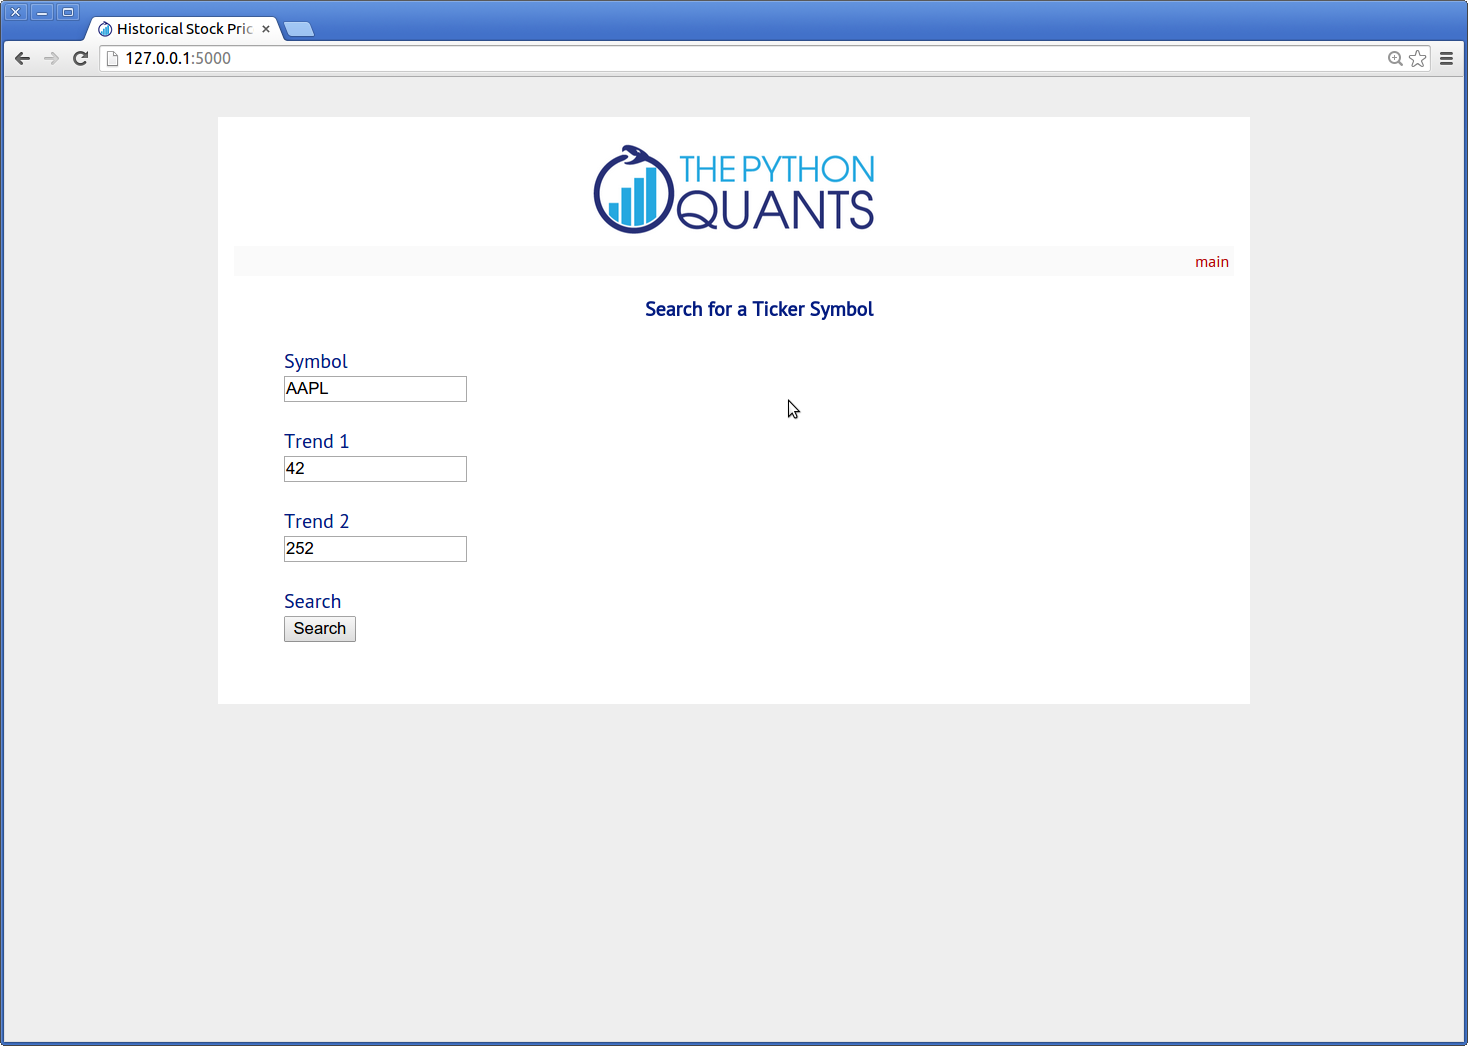
\includegraphics{stock_app_main.png}}

The \textbf{results output page} looks like this:

\scalebox{0.660000}{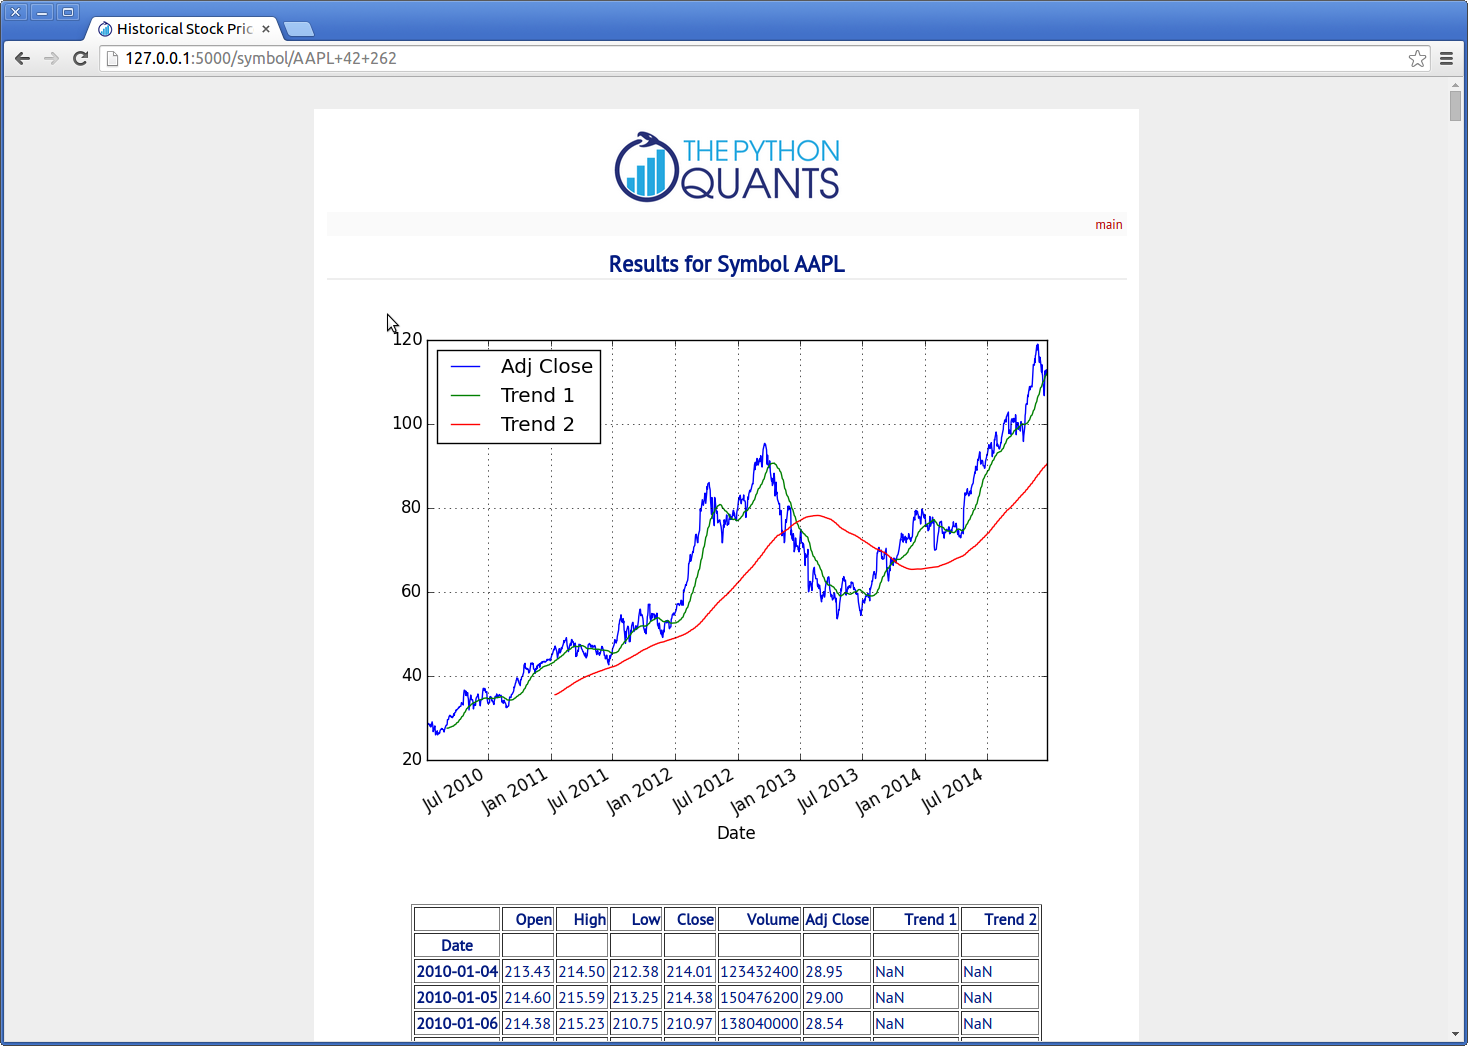
\includegraphics{stock_app_results.png}}


\subsection{Generating Interactive D3 Plots}
\label{03_web_apps:generating-interactive-d3-plots}
Modern Web applications generally rely on nicely rendered, interactive graphics. The following example slightly adjusts the previous one to accomplish exaclty that. The main tool used here is \textbf{plotly} (cf. \href{http://plot.ly}{http://plot.ly}), a graphics engine that allows to easily transform static Python/matplotlib plots into interactive \textbf{D3.js} plots (\href{http://d3js.org/}{http://d3js.org/}).

You need to \textbf{install plotly} as follows:

\begin{Verbatim}[commandchars=\\\{\}]
sudo pip install plotly
\end{Verbatim}

You also need to create an account on the Web site \href{http://plot.ly}{http://plot.ly}.

The major \textbf{changes} have be made in the main application module (\code{download link}):

\begin{Verbatim}[commandchars=\\\{\}]
\PYG{c}{\PYGZsh{}}
\PYG{c}{\PYGZsh{} Historical Stock Prices}
\PYG{c}{\PYGZsh{} with the RPi using Python \PYGZam{} Flask \PYGZam{} Plotly}
\PYG{c}{\PYGZsh{}}
\PYG{c}{\PYGZsh{} stock\PYGZus{}interactive.py}
\PYG{c}{\PYGZsh{}}
\PYG{c}{\PYGZsh{} (c) Dr. Yves J. Hilpisch}
\PYG{c}{\PYGZsh{} The Python Quants}
\PYG{c}{\PYGZsh{}}

\PYG{k+kn}{import} \PYG{n+nn}{pandas} \PYG{k+kn}{as} \PYG{n+nn}{pd}
\PYG{k+kn}{import} \PYG{n+nn}{pandas.io.data} \PYG{k+kn}{as} \PYG{n+nn}{web}
\PYG{k+kn}{import} \PYG{n+nn}{matplotlib.pyplot} \PYG{k+kn}{as} \PYG{n+nn}{plt}
\PYG{k+kn}{import} \PYG{n+nn}{plotly.plotly} \PYG{k+kn}{as} \PYG{n+nn}{ply}
\PYG{k+kn}{from} \PYG{n+nn}{plotly.graph\PYGZus{}objs} \PYG{k+kn}{import} \PYG{n}{Figure}\PYG{p}{,} \PYG{n}{Layout}\PYG{p}{,} \PYG{n}{XAxis}\PYG{p}{,} \PYG{n}{YAxis}
\PYG{k+kn}{from} \PYG{n+nn}{flask} \PYG{k+kn}{import} \PYG{n}{Flask}\PYG{p}{,} \PYG{n}{request}\PYG{p}{,} \PYG{n}{render\PYGZus{}template}\PYG{p}{,} \PYG{n}{redirect}\PYG{p}{,} \PYG{n}{url\PYGZus{}for}
\PYG{k+kn}{from} \PYG{n+nn}{forms} \PYG{k+kn}{import} \PYG{n}{SymbolSearch}

\PYG{c}{\PYGZsh{}}
\PYG{c}{\PYGZsh{} Needed for plotly usage}
\PYG{c}{\PYGZsh{}}

\PYG{n}{ply}\PYG{o}{.}\PYG{n}{sign\PYGZus{}in}\PYG{p}{(}\PYG{l+s}{\PYGZsq{}}\PYG{l+s}{yves}\PYG{l+s}{\PYGZsq{}}\PYG{p}{,} \PYG{l+s}{\PYGZsq{}}\PYG{l+s}{65p6tn4p8i}\PYG{l+s}{\PYGZsq{}}\PYG{p}{)}

\PYG{k}{def} \PYG{n+nf}{df\PYGZus{}to\PYGZus{}plotly}\PYG{p}{(}\PYG{n}{df}\PYG{p}{)}\PYG{p}{:}
    \PYG{l+s+sd}{\PYGZsq{}\PYGZsq{}\PYGZsq{}}
\PYG{l+s+sd}{    Converting a pandas DataFrame to plotly compatible format.}
\PYG{l+s+sd}{    \PYGZsq{}\PYGZsq{}\PYGZsq{}}
    \PYG{k}{if} \PYG{n}{df}\PYG{o}{.}\PYG{n}{index}\PYG{o}{.}\PYG{n}{\PYGZus{}\PYGZus{}class\PYGZus{}\PYGZus{}}\PYG{o}{.}\PYG{n}{\PYGZus{}\PYGZus{}name\PYGZus{}\PYGZus{}}\PYG{o}{==}\PYG{l+s}{\PYGZdq{}}\PYG{l+s}{DatetimeIndex}\PYG{l+s}{\PYGZdq{}}\PYG{p}{:}
        \PYG{n}{x} \PYG{o}{=} \PYG{n}{df}\PYG{o}{.}\PYG{n}{index}\PYG{o}{.}\PYG{n}{format}\PYG{p}{(}\PYG{p}{)}
    \PYG{k}{else}\PYG{p}{:}
        \PYG{n}{x} \PYG{o}{=} \PYG{n}{df}\PYG{o}{.}\PYG{n}{index}\PYG{o}{.}\PYG{n}{values} 
    \PYG{n}{lines} \PYG{o}{=} \PYG{p}{\PYGZob{}}\PYG{p}{\PYGZcb{}}
    \PYG{k}{for} \PYG{n}{key} \PYG{o+ow}{in} \PYG{n}{df}\PYG{p}{:}
        \PYG{n}{lines}\PYG{p}{[}\PYG{n}{key}\PYG{p}{]} \PYG{o}{=} \PYG{p}{\PYGZob{}}\PYG{p}{\PYGZcb{}}
        \PYG{n}{lines}\PYG{p}{[}\PYG{n}{key}\PYG{p}{]}\PYG{p}{[}\PYG{l+s}{\PYGZsq{}}\PYG{l+s}{x}\PYG{l+s}{\PYGZsq{}}\PYG{p}{]} \PYG{o}{=} \PYG{n}{x}
        \PYG{n}{lines}\PYG{p}{[}\PYG{n}{key}\PYG{p}{]}\PYG{p}{[}\PYG{l+s}{\PYGZsq{}}\PYG{l+s}{y}\PYG{l+s}{\PYGZsq{}}\PYG{p}{]} \PYG{o}{=} \PYG{n}{df}\PYG{p}{[}\PYG{n}{key}\PYG{p}{]}\PYG{o}{.}\PYG{n}{values}
        \PYG{n}{lines}\PYG{p}{[}\PYG{n}{key}\PYG{p}{]}\PYG{p}{[}\PYG{l+s}{\PYGZsq{}}\PYG{l+s}{name}\PYG{l+s}{\PYGZsq{}}\PYG{p}{]} \PYG{o}{=} \PYG{n}{key}
    \PYG{n}{lines\PYGZus{}plotly} \PYG{o}{=} \PYG{p}{[}\PYG{n}{lines}\PYG{p}{[}\PYG{n}{key}\PYG{p}{]} \PYG{k}{for} \PYG{n}{key} \PYG{o+ow}{in} \PYG{n}{df}\PYG{p}{]}
    \PYG{k}{return} \PYG{n}{lines\PYGZus{}plotly}

\PYG{c}{\PYGZsh{}}
\PYG{c}{\PYGZsh{} Main app}
\PYG{c}{\PYGZsh{}}

\PYG{n}{app} \PYG{o}{=} \PYG{n}{Flask}\PYG{p}{(}\PYG{n}{\PYGZus{}\PYGZus{}name\PYGZus{}\PYGZus{}}\PYG{p}{)}

\PYG{n+nd}{@app.route}\PYG{p}{(}\PYG{l+s}{\PYGZdq{}}\PYG{l+s}{/}\PYG{l+s}{\PYGZdq{}}\PYG{p}{,} \PYG{n}{methods}\PYG{o}{=}\PYG{p}{[}\PYG{l+s}{\PYGZsq{}}\PYG{l+s}{GET}\PYG{l+s}{\PYGZsq{}}\PYG{p}{,} \PYG{l+s}{\PYGZsq{}}\PYG{l+s}{POST}\PYG{l+s}{\PYGZsq{}}\PYG{p}{]}\PYG{p}{)}
\PYG{k}{def} \PYG{n+nf}{main}\PYG{p}{(}\PYG{p}{)}\PYG{p}{:}
    \PYG{n}{form} \PYG{o}{=} \PYG{n}{SymbolSearch}\PYG{p}{(}\PYG{n}{csrf\PYGZus{}enabled}\PYG{o}{=}\PYG{n+nb+bp}{False}\PYG{p}{)}
    \PYG{k}{if} \PYG{n}{request}\PYG{o}{.}\PYG{n}{method} \PYG{o}{==} \PYG{l+s}{\PYGZsq{}}\PYG{l+s}{POST}\PYG{l+s}{\PYGZsq{}}\PYG{p}{:}
        \PYG{k}{return} \PYG{n}{redirect}\PYG{p}{(}\PYG{n}{url\PYGZus{}for}\PYG{p}{(}\PYG{l+s}{\PYGZsq{}}\PYG{l+s}{results}\PYG{l+s}{\PYGZsq{}}\PYG{p}{,} \PYG{n}{symbol}\PYG{o}{=}\PYG{n}{request}\PYG{o}{.}\PYG{n}{form}\PYG{p}{[}\PYG{l+s}{\PYGZsq{}}\PYG{l+s}{symbol}\PYG{l+s}{\PYGZsq{}}\PYG{p}{]}\PYG{p}{,}
                            \PYG{n}{trend1}\PYG{o}{=}\PYG{n}{request}\PYG{o}{.}\PYG{n}{form}\PYG{p}{[}\PYG{l+s}{\PYGZsq{}}\PYG{l+s}{trend1}\PYG{l+s}{\PYGZsq{}}\PYG{p}{]}\PYG{p}{,}
                            \PYG{n}{trend2}\PYG{o}{=}\PYG{n}{request}\PYG{o}{.}\PYG{n}{form}\PYG{p}{[}\PYG{l+s}{\PYGZsq{}}\PYG{l+s}{trend2}\PYG{l+s}{\PYGZsq{}}\PYG{p}{]}\PYG{p}{)}\PYG{p}{)}
    \PYG{k}{return} \PYG{n}{render\PYGZus{}template}\PYG{p}{(}\PYG{l+s}{\PYGZsq{}}\PYG{l+s}{selection.html}\PYG{l+s}{\PYGZsq{}}\PYG{p}{,} \PYG{n}{form}\PYG{o}{=}\PYG{n}{form}\PYG{p}{)}

\PYG{n+nd}{@app.route}\PYG{p}{(}\PYG{l+s}{\PYGZdq{}}\PYG{l+s}{/symbol/\PYGZlt{}symbol\PYGZgt{}+\PYGZlt{}trend1\PYGZgt{}+\PYGZlt{}trend2\PYGZgt{}}\PYG{l+s}{\PYGZdq{}}\PYG{p}{)}
\PYG{k}{def} \PYG{n+nf}{results}\PYG{p}{(}\PYG{n}{symbol}\PYG{p}{,} \PYG{n}{trend1}\PYG{p}{,} \PYG{n}{trend2}\PYG{p}{)}\PYG{p}{:}
    \PYG{n}{data} \PYG{o}{=} \PYG{n}{web}\PYG{o}{.}\PYG{n}{DataReader}\PYG{p}{(}\PYG{n}{symbol}\PYG{p}{,} \PYG{n}{data\PYGZus{}source}\PYG{o}{=}\PYG{l+s}{\PYGZsq{}}\PYG{l+s}{yahoo}\PYG{l+s}{\PYGZsq{}}\PYG{p}{)}
    \PYG{n}{data}\PYG{p}{[}\PYG{l+s}{\PYGZsq{}}\PYG{l+s}{Trend 1}\PYG{l+s}{\PYGZsq{}}\PYG{p}{]} \PYG{o}{=} \PYG{n}{pd}\PYG{o}{.}\PYG{n}{rolling\PYGZus{}mean}\PYG{p}{(}\PYG{n}{data}\PYG{p}{[}\PYG{l+s}{\PYGZsq{}}\PYG{l+s}{Adj Close}\PYG{l+s}{\PYGZsq{}}\PYG{p}{]}\PYG{p}{,} \PYG{n}{window}\PYG{o}{=}\PYG{n+nb}{int}\PYG{p}{(}\PYG{n}{trend1}\PYG{p}{)}\PYG{p}{)}
    \PYG{n}{data}\PYG{p}{[}\PYG{l+s}{\PYGZsq{}}\PYG{l+s}{Trend 2}\PYG{l+s}{\PYGZsq{}}\PYG{p}{]} \PYG{o}{=} \PYG{n}{pd}\PYG{o}{.}\PYG{n}{rolling\PYGZus{}mean}\PYG{p}{(}\PYG{n}{data}\PYG{p}{[}\PYG{l+s}{\PYGZsq{}}\PYG{l+s}{Adj Close}\PYG{l+s}{\PYGZsq{}}\PYG{p}{]}\PYG{p}{,} \PYG{n}{window}\PYG{o}{=}\PYG{n+nb}{int}\PYG{p}{(}\PYG{n}{trend2}\PYG{p}{)}\PYG{p}{)}
    \PYG{n}{layout} \PYG{o}{=} \PYG{n}{Layout}\PYG{p}{(}
        \PYG{n}{xaxis}\PYG{o}{=}\PYG{n}{XAxis}\PYG{p}{(}\PYG{n}{showgrid}\PYG{o}{=}\PYG{n+nb+bp}{True}\PYG{p}{,} \PYG{n}{gridcolor}\PYG{o}{=}\PYG{l+s}{\PYGZsq{}}\PYG{l+s}{\PYGZsh{}bdbdbd}\PYG{l+s}{\PYGZsq{}}\PYG{p}{,} \PYG{n}{gridwidth}\PYG{o}{=}\PYG{l+m+mi}{2}\PYG{p}{)}\PYG{p}{,}
        \PYG{n}{yaxis}\PYG{o}{=}\PYG{n}{YAxis}\PYG{p}{(}\PYG{n}{showgrid}\PYG{o}{=}\PYG{n+nb+bp}{True}\PYG{p}{,} \PYG{n}{gridcolor}\PYG{o}{=}\PYG{l+s}{\PYGZsq{}}\PYG{l+s}{\PYGZsh{}bdbdbd}\PYG{l+s}{\PYGZsq{}}\PYG{p}{,} \PYG{n}{gridwidth}\PYG{o}{=}\PYG{l+m+mi}{2}\PYG{p}{)}
    \PYG{p}{)}
    \PYG{n}{fig} \PYG{o}{=} \PYG{n}{Figure}\PYG{p}{(}\PYG{n}{data}\PYG{o}{=}\PYG{n}{df\PYGZus{}to\PYGZus{}plotly}\PYG{p}{(}\PYG{n}{data}\PYG{p}{[}\PYG{p}{[}\PYG{l+s}{\PYGZsq{}}\PYG{l+s}{Adj Close}\PYG{l+s}{\PYGZsq{}}\PYG{p}{,} \PYG{l+s}{\PYGZsq{}}\PYG{l+s}{Trend 1}\PYG{l+s}{\PYGZsq{}}\PYG{p}{,} \PYG{l+s}{\PYGZsq{}}\PYG{l+s}{Trend 2}\PYG{l+s}{\PYGZsq{}}\PYG{p}{]}\PYG{p}{]}\PYG{p}{)}\PYG{p}{,}
                \PYG{n}{layout}\PYG{o}{=}\PYG{n}{layout}\PYG{p}{)}
    \PYG{n}{plot} \PYG{o}{=} \PYG{n}{ply}\PYG{o}{.}\PYG{n}{plot}\PYG{p}{(}\PYG{n}{fig}\PYG{p}{,} \PYG{n}{auto\PYGZus{}open}\PYG{o}{=}\PYG{n+nb+bp}{False}\PYG{p}{)}
    \PYG{n}{table} \PYG{o}{=} \PYG{n}{data}\PYG{o}{.}\PYG{n}{to\PYGZus{}html}\PYG{p}{(}\PYG{p}{)}
    \PYG{k}{return} \PYG{n}{render\PYGZus{}template}\PYG{p}{(}\PYG{l+s}{\PYGZsq{}}\PYG{l+s}{plotly.html}\PYG{l+s}{\PYGZsq{}}\PYG{p}{,} \PYG{n}{symbol}\PYG{o}{=}\PYG{n}{symbol}\PYG{p}{,}
                            \PYG{n}{plot}\PYG{o}{=}\PYG{n}{plot}\PYG{p}{,} \PYG{n}{table}\PYG{o}{=}\PYG{n}{table}\PYG{p}{)}


\PYG{k}{if} \PYG{n}{\PYGZus{}\PYGZus{}name\PYGZus{}\PYGZus{}} \PYG{o}{==} \PYG{l+s}{\PYGZsq{}}\PYG{l+s}{\PYGZus{}\PYGZus{}main\PYGZus{}\PYGZus{}}\PYG{l+s}{\PYGZsq{}}\PYG{p}{:}
    \PYG{n}{app}\PYG{o}{.}\PYG{n}{run}\PYG{p}{(}\PYG{n}{debug}\PYG{o}{=}\PYG{n+nb+bp}{True}\PYG{p}{)}
\end{Verbatim}

We also need to \textbf{adjust the results output template file} (\code{download link}):

\begin{Verbatim}[commandchars=\\\{\}]
\PYG{c}{\PYGZlt{}!\PYGZhy{}\PYGZhy{}}\PYG{c}{ plotly.html }\PYG{c}{\PYGZhy{}\PYGZhy{}\PYGZgt{}}
\PYGZob{}\PYGZpc{} extends \PYGZdq{}layout.html\PYGZdq{} \PYGZpc{}\PYGZcb{}

\PYGZob{}\PYGZpc{} block body \PYGZpc{}\PYGZcb{}


    \PYG{n+nt}{\PYGZlt{}h1}\PYG{n+nt}{\PYGZgt{}}Results for Symbol \PYGZob{}\PYGZob{} symbol \PYGZcb{}\PYGZcb{}\PYG{n+nt}{\PYGZlt{}/h1\PYGZgt{}}

    \PYG{n+nt}{\PYGZlt{}iframe}

    \PYG{n+na}{width=}\PYG{l+s}{100\PYGZpc{}} \PYG{n+na}{height=}\PYG{l+s}{\PYGZdq{}650\PYGZdq{}} \PYG{n+na}{frameborder=}\PYG{l+s}{\PYGZdq{}0\PYGZdq{}} \PYG{n+na}{seamless=}\PYG{l+s}{\PYGZdq{}seamless\PYGZdq{}} \PYG{n+na}{scrolling=}\PYG{l+s}{\PYGZdq{}no\PYGZdq{}}

    \PYG{n+na}{src=}\PYG{l+s}{\PYGZdq{}\PYGZob{}\PYGZob{} plot \PYGZcb{}\PYGZcb{}.embed?width=100\PYGZpc{}\PYGZam{}height=650\PYGZdq{}}\PYG{n+nt}{\PYGZgt{}}

    \PYG{n+nt}{\PYGZlt{}/iframe\PYGZgt{}}

    \PYG{n+nt}{\PYGZlt{}br}\PYG{n+nt}{\PYGZgt{}}\PYG{n+nt}{\PYGZlt{}br}\PYG{n+nt}{\PYGZgt{}}

    \PYGZob{}\PYGZob{} table \textbar{} safe \PYGZcb{}\PYGZcb{}


\PYGZob{}\PYGZpc{} endblock \PYGZpc{}\PYGZcb{}
\end{Verbatim}

Also, the \textbf{WSGI wrapping} is to be adjusted slightly (\code{download link}):

\begin{Verbatim}[commandchars=\\\{\}]
\PYG{c}{\PYGZsh{}}
\PYG{c}{\PYGZsh{} WSGI Wrapper for the}
\PYG{c}{\PYGZsh{} Historical Stock Data App (Interactive)}
\PYG{c}{\PYGZsh{}}
\PYG{c}{\PYGZsh{} run\PYGZus{}stock\PYGZus{}int.py}
\PYG{c}{\PYGZsh{} }
\PYG{k+kn}{from} \PYG{n+nn}{tornado.wsgi} \PYG{k+kn}{import} \PYG{n}{WSGIContainer}
\PYG{k+kn}{from} \PYG{n+nn}{tornado.httpserver} \PYG{k+kn}{import} \PYG{n}{HTTPServer}
\PYG{k+kn}{from} \PYG{n+nn}{tornado.ioloop} \PYG{k+kn}{import} \PYG{n}{IOLoop}
\PYG{k+kn}{from} \PYG{n+nn}{stock\PYGZus{}interactive} \PYG{k+kn}{import} \PYG{n}{app}

\PYG{n}{http\PYGZus{}server} \PYG{o}{=} \PYG{n}{HTTPServer}\PYG{p}{(}\PYG{n}{WSGIContainer}\PYG{p}{(}\PYG{n}{app}\PYG{p}{)}\PYG{p}{)}
\PYG{n}{http\PYGZus{}server}\PYG{o}{.}\PYG{n}{listen}\PYG{p}{(}\PYG{l+m+mi}{8888}\PYG{p}{)}  \PYG{c}{\PYGZsh{} serving on port 8888}
\PYG{n}{IOLoop}\PYG{o}{.}\PYG{n}{instance}\PYG{p}{(}\PYG{p}{)}\PYG{o}{.}\PYG{n}{start}\PYG{p}{(}\PYG{p}{)}
\end{Verbatim}

Everything else remains the same. Your \textbf{folder structure} should now look like follows:

\begin{Verbatim}[commandchars=\\\{\}]
\PYG{g+gp}{In [3]: }\PYG{k}{for} \PYG{n}{path}\PYG{p}{,} \PYG{n}{dirs}\PYG{p}{,} \PYG{n}{files} \PYG{o+ow}{in} \PYG{n}{os}\PYG{o}{.}\PYG{n}{walk}\PYG{p}{(}\PYG{l+s}{\PYGZsq{}}\PYG{l+s}{./source/stock\PYGZus{}int}\PYG{l+s}{\PYGZsq{}}\PYG{p}{)}\PYG{p}{:}
\PYG{g+gp}{   ...: }    \PYG{k}{print} \PYG{n}{path}
\PYG{g+gp}{   ...: }    \PYG{k}{for} \PYG{n}{f} \PYG{o+ow}{in} \PYG{n}{files}\PYG{p}{:}
\PYG{g+gp}{   ...: }        \PYG{k}{print} \PYG{n}{f}
\PYG{g+gp}{   ...: }
\PYG{g+go}{./source/stock\PYGZus{}int}
\PYG{g+go}{forms.py}
\PYG{g+go}{run\PYGZus{}stock\PYGZus{}int.py}
\PYG{g+go}{stock\PYGZus{}interactive.py}
\PYG{g+go}{./source/stock\PYGZus{}int/static}
\PYG{g+go}{style.css}
\PYG{g+go}{./source/stock\PYGZus{}int/templates}
\PYG{g+go}{layout.html}
\PYG{g+go}{plotly.html}
\PYG{g+go}{selection.html}
\end{Verbatim}

If everything runs as desired, the \textbf{results page} of the interactive version should look like below (here the app runs locally):

\scalebox{0.660000}{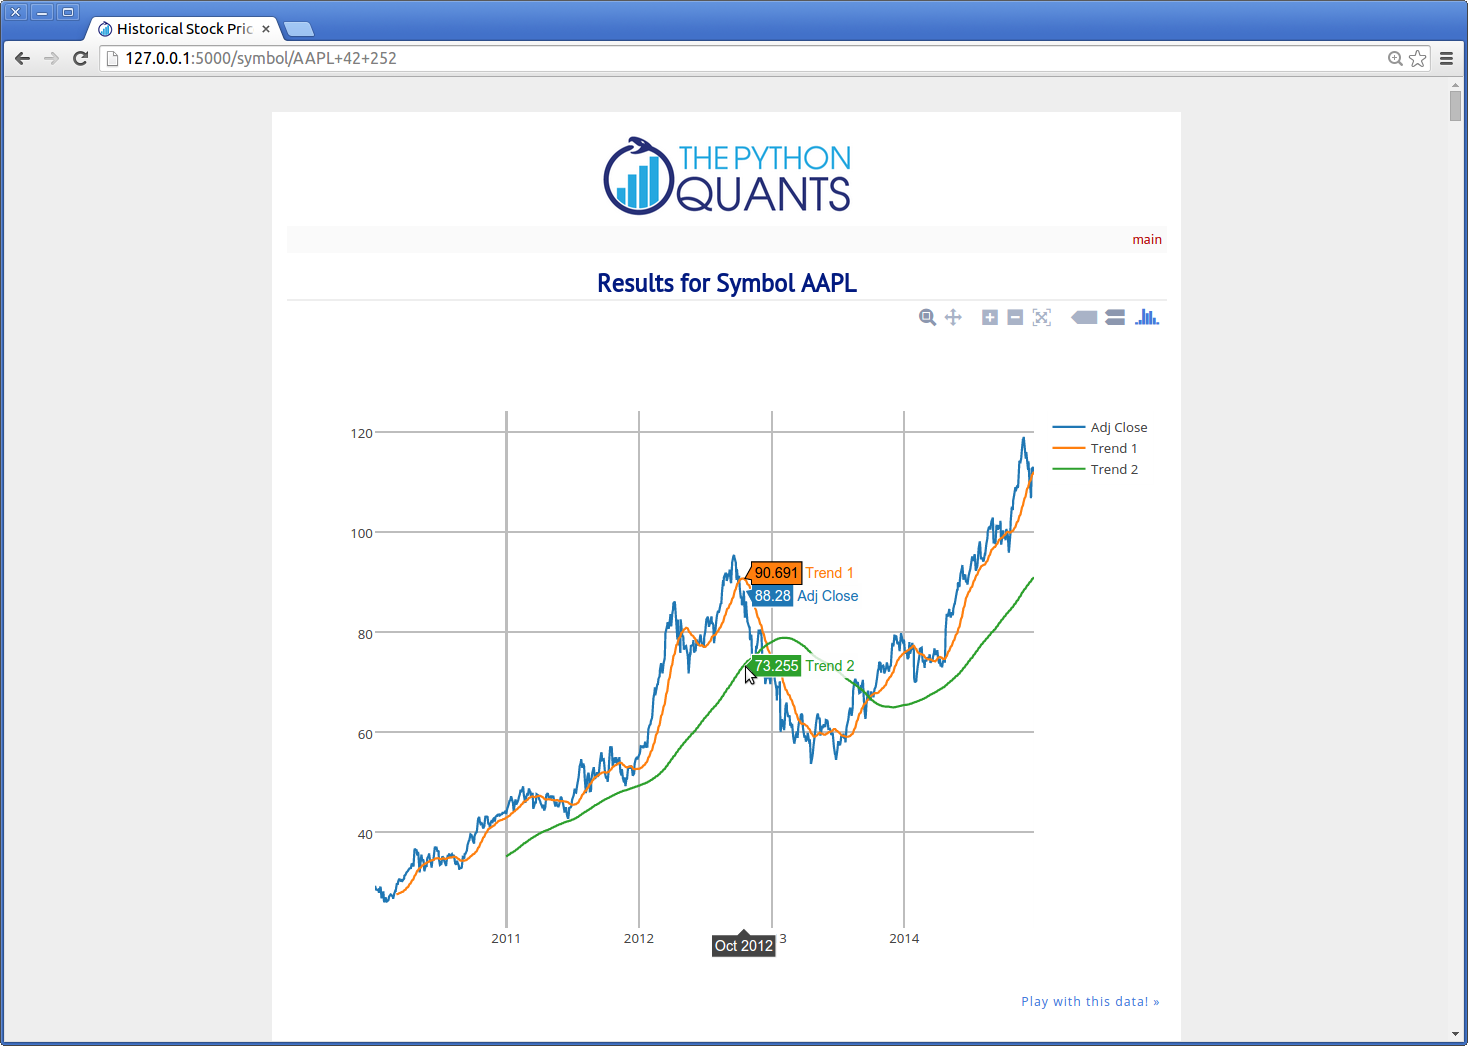
\includegraphics{stock_app_plotly.png}}


\chapter{About the Author}
\label{index:about-the-author}
Yves Hilpisch is managing partner of The Python Quants GmbH (Germany) and co-founder of The Python Quants LLC (New York City). The Python Quants provide, among others, the \textbf{Python Quant Platform} as a solution for browser-based, interactive, collaborative financial analytics (cf. \href{http://quant-platform.com}{http://quant-platform.com}). On this platform (for which free trials are available) you can also immediately try our open source financial analytics library DX Analytics (\href{http://dx-analytics.com}{http://dx-analytics.com}).


\chapter{Copyright \& Disclaimer}
\label{index:copyright-disclaimer}
© Dr. Yves J. Hilpisch \textbar{} The Python Quants GmbH

This Web site comes with no representations or warranties, to the extent
permitted by applicable law.

\href{http://www.pythonquants.com}{http://www.pythonquants.com} \textbar{} \href{mailto:rpi@pythonquants.com}{rpi@pythonquants.com} \textbar{}
\href{http://twitter.com/dyjh}{http://twitter.com/dyjh}

\textbf{Python Quant Platform} \textbar{} \href{http://quant-platform.com}{http://quant-platform.com}

\textbf{Derivatives Analytics with Python (Wiley Finance)} \textbar{}
\href{http://eu.wiley.com/WileyCDA/WileyTitle/productCd-1119037999.html}{http://eu.wiley.com/WileyCDA/WileyTitle/productCd-1119037999.html}

\textbf{Python for Finance (O'Reilly)} \textbar{}
\href{http://shop.oreilly.com/product/0636920032441.do}{http://shop.oreilly.com/product/0636920032441.do}



\renewcommand{\indexname}{Index}
\printindex
\end{document}
